\documentclass[12pt,a4paper,notitlepage]{report}
%\usepackage[ngerman,french,english]{babel}
\usepackage[utf8]{inputenc}
\usepackage{pdfpages} % to prepend the title page
\usepackage{amsfonts}
\usepackage{amsmath}
\usepackage{subcaption}  % not sure if this is necessary
\usepackage[skip=10pt plus1pt, indent=0pt]{parskip} % skip space after paragraph and remove indent
\usepackage{csvsimple}
\usepackage{booktabs}
\usepackage{floatrow}
\usepackage{tocloft}
\usepackage[font={sf, small,it}]{caption} % change caption appearance
\usepackage{titlesec}
\usepackage[scaled]{helvet} % Scale Helvetica to match the size of the default font
\usepackage[T1]{fontenc}    % Ensure proper font encoding
\usepackage{lmodern}
\usepackage[backend=biber, style=apa, url=false, sorting=ynt]{biblatex} % citations
\usepackage{graphicx} % for images
\graphicspath{ {./images/} }

\renewcommand{\familydefault}{\sfdefault} % Set the default font to sans-serif (Helvetica)

\emergencystretch=2em % if a line is too long, allow 2em over

% code snippets style
\usepackage{listings}
\usepackage{xcolor}
\definecolor{bg}{HTML}{EEE5E9}
\definecolor{orange}{HTML}{CF5C36}
\definecolor{gray}{HTML}{7C7C7C}
\definecolor{codegray}{rgb}{0.5,0.5,0.5}
\definecolor{codepurple}{rgb}{0.58,0,0.82}
\lstdefinestyle{python}{
  basewidth={.5em,0.4em},
  backgroundcolor=\color{bg},   
  commentstyle=\color{gray},
  keywordstyle=\color{orange},
  numberstyle=\tiny\color{codegray},
  stringstyle=\color{codepurple},
  basicstyle=\ttfamily\footnotesize,
  breakatwhitespace=false,         
  breaklines=true,                 
  captionpos=b,                    
  keepspaces=true,                 
  numbers=left,                    
  numbersep=5pt,                  
  showspaces=false,                
  showstringspaces=false,
  showtabs=false,                  
  tabsize=4,
  %frame=shadowbox,
  xleftmargin=2em,
  frame=single,
  framexleftmargin=1.5em
}
\lstset{style=python}

% define headline styles
\titleformat{\chapter}[display]
  {\normalfont\sffamily\huge\bfseries}
  {\chaptertitlename\ \thechapter}{0pt}{\Huge}
\titleformat{\section}
  {\normalfont\sffamily\Large\bfseries}
  {\thesection}{1em}{}
\titleformat{\subsection}
  {\normalfont\sffamily\Large}
  {\thesubsection}{1em}{}
\titleformat{\subsubsection}
  {\normalfont\sffamily\large}
  {\thesubsubsection}{1em}{}

\addbibresource{bibliography.bib}

\addbibresource{bibliography.bib}


\begin{document}
\sffamily


% Title Page
\begin{titlepage}
\normalfont\sffamily \centering

\includegraphics[width=5.7cm]{logo.png}
\begin{center}
\vspace*{1cm}
\LARGE{Masters Thesis}\\
\vspace*{1cm}
\huge\textbf{Winning the Lottery Twice}\\
\large\vspace*{2cm}
\textbf{zur Erlangung des akademischen Grades}\\
Master of Science (MSc) \\
\vspace*{1cm}
\textbf{an der \\ Johannes Kepler Universität Linz}\\
Institut für Machine Learning\\
\vspace{1cm}
\textbf{unter der Anleitung von:} \\
Assoc.Prof.\ Mag.\ Dr.\ Günter Klambauer\\
Dipl.-Ing. Pieter-Jan Hoedt \\
\vspace{1cm}
\textbf{eingereicht von:} \\
Maximilian Burger, BSc.\\
\vspace{1cm}
Linz, 04. März 2024
\end{center}
\end{titlepage}

% Thesis requirements
\pagenumbering{roman}
\chapter*{Erklärung}
Danke
\chapter*{Preamble}

Add preamble

% start of the thesis
\pagenumbering{arabic}
\chapter*{Abstract}
\addcontentsline{toc}{chapter}{Abstract}

The \textbf{Lottery Ticket Hypothesis} by \textcite{LTH} has sparked a novel field of research that concerns itself with well-trainable sparse neural networks.
One key method in this field is called \textit{Iterative Magnitude Pruning}, which is successful in finding sparse subnetworks that can be trained to high performance. These networks are called \textit{Winning Tickets}.
Many aspects of why and how this procedure works and what characteristics of the winning tickets make them successful remain elusive.
One way to learn more about lottery tickets would be to study their network structure.
Since they are usually highly sparse, their structure may contain valuable insights into their functionality.
In this thesis, the structure of winning ticket networks is analyzed and how it relates to the data the network was trained on.
The experiments in this thesis are conducted on datasets that contain two independent tasks \rule[0.5ex]{.5em}{0.5pt} a simple toy dataset and a combination of the MNIST and Fashion-MNIST datasets.
On both datasets, winning tickets derived with iterative magnitude pruning are found that contain separate, independent subnetworks where each subnetwork solves one task.

\chapter*{Kurzfassung}
\addcontentsline{toc}{chapter}{Kurzfassung}

Die von \textcite{LTH} aufgestellte \textbf{Lottery Ticket Hypothese} hat einen neuen Teilbereich der Forschung begründet, der sich mit `Sparse Neural Networks' beschäftigt.
`Iterative Magnitude Pruning' (IMP) ist eine Schlüsselmethode für dieses Feld, da sie die schlanken und performanten Subnetzwerke, die sogenannten \textit{Winning Tickets} erfolgreich ausfindig machen kann.
Jedoch sind viele Aspekte der Funktionsweise dieser Technik noch unerklärt.
Eine Möglichkeit um \textit{Winning Tickets} und deren Erzeugung besser zu verstehen, ist die Analyse des Netzwerkgraphens.
Dadurch, dass \textit{Winning Tickets} `sparse' sind, könnte ihre Struktur wertvolle Einblicke in die Funktion des Netzwerkes bieten.
Um mehr über die Struktur dieser Netze zu erfahren wurden Experimente durchgeführt, welche von \textcite{BIMT} inspiriert wurden.
Ein Datensatz, welcher zwei voneinander unabhängige Aufgaben enthält, wurde genutzt, um mittels \textit{IMP} Subnetze zu finden.
Folgende Frage wird in dieser Arbeit gestellt:
Enthält das \textit{Winning Ticket} zwei unabhängige Subnetzte, eines für jede Aufgabe?
\newpage

% start of the main part
\tableofcontents
\chapter{Introduction}
Neural Networks have achieved remarkable success in various tasks, however, their increasingly large size leads to high computational and memory requirements.
Neural Network Pruning \autocite{LeCun, OptimalBrainSurgeon, HanEtAl15, PruningFiltersForEfficientConvets} has been proposed to reduce the number of parameters after the network is trained, while maintaining accuracy.
This leads to a reduction in size \autocite{HanEtAl15} and energy consumption \autocite{YangCS17} in the resulting subnetworks during inference.

To increase efficiency during training as well, the smaller networks need to be trained from the beginning. Attempts to train smaller networks discovered by pruning from scratch did not yield convincing results \autocite{HanEtAl15, PruningFiltersForEfficientConvets}.

The Lottery Ticket Hypothesis by \textcite{LTH} has shown that there exist small, well-initialized subnetworks that can be trained in isolation to reach the same accuracy as the unpruned networks. 
In contrast to previous attempts where the subnetwork structure after pruning is randomly reinitialized \autocite{HanEtAl15, PruningFiltersForEfficientConvets}, \textcite{LTH} reinitialize the subnetworks with their respective initial weights from before training.
The subnetwork structure is uncovered by an algorithm called Iterative Magnitude Pruning (IMP).
Different approaches for discovering small, well-performing subnetworks were developed \autocite{Supermasks}, Edge Popup \autocite{DBLP:conf/cvpr/RamanujanWKFR20}, and Gem-Miner\autocite{RareGems}.

However, the structure of the underlying sparse subnetwork is rarely discussed.
Since the networks are sparse, often to a high degree, the structure might give valuable insights into the functionality of the subnetwork.
Yet, analysing the structure of network is not an easy undertaking.

To generate insights about the structure of lottery tickets, the problem is approach from the other side.
One could take a problem with a known structure and test if the resulting sparse networks resembles that structure in a way.
For instance, given a problem that consists of two independent subproblems may result in two independent subnetworks. 
One for each subproblem, or task.

\section{Motivation}
The study of lottery tickets itself has broad ramifications.
At its ultimate, it could reduce the size of the neural networks significantly during training.
This would result in lower computational and memory requirements and therefore cost and energy savings.
It could also enable us to train models larger than prevousily possible, due to an increased efficiency of each parameter.
Studying the structure of lottery tickets might produce valuable insights that further advance the field.

Further, since the lottery tickets are highly sparse, they represent a very reduced function that solves the problem.
This might turn out valuable for network interpretation.
The structure of the network might yield information about how the network solves a task.
This could enrich the current ecosystem of techniques to interpret neural networks.

\section{Structure of the Thesis}
In the first section a literature review is conducted, where relevant topics to this thesis are described.

The next chapter explains the methodology.
The dataset, neural network architecture and training process is outlined, as well as other algorithms used in the experiments.
The following chapter walks through the conducted expirements.
It contains the experiment setup, the results and interpretation of those.
The thesis is concluded with a discussion of of future research in this direction.
\chapter{Literature Review}

overparameterization: [3] Yann Dauphin and Yoshua Bengio. Big neural networks waste capacity. CoRR, abs/1301.3583, 2013.

Misha Denil, Babak Shakibi, Laurent Dinh, Nando de Freitas, et al. Predicting parameters in deep learning. In Advances in Neural Information Processing Systems, pages 2148-2156, 2013.

Great intro to compression in Zhou et al Supermasks.

TODO introduction to the literature review  
at the core this thesis is about understanding the structure of lottery tickets. So what is or was important about that?
\begin{itemize}
    \item lottery ticket Hypothesis, its relevance 
    \item derivative works of the lth, attempts to understand it
    \item structure of lottery tickets? is there really nothing? connectedness, degree (original LTH), Han et al says there will be dead neurons, All allive pruning says they kill them
    \item understanding networks, mechanistic interpretability, independence as a nice thing to understand stuff. Bimt showing independece is in the network
\end{itemize}

Is the structure of the lottery ticket useful? interpretable? or is it merely super overfitted random shit that doesnt help you anyway.

\section{Deep Learning}
The field of deep learning is largely responsible for the advances of modern machine learning applications.
With increasing amounts of available data and computational resources, the size of neural networks has increased drastically, as well as their performance.
However, this increase in size poses challenges in constrained environements.
Larger and deeper networks tend to require more memory and compute, which can be problematic for inference on constrained devices.
Also, larger models typically require more time and more energy for training as well as for inference.
Neural Network Pruning \autocite{LeCun, OptimalBrainSurgeon, HanEtAl15, PruningFiltersForEfficientConvets} has been proposed as a tool to reduce network size for inference, while maintaining accuracy.

\section{Neural Network Pruning}
Neural Network Pruning is a category of methods that eliminate components of the network whilst aiming to minimally impact its performance.
Pruning algorithms can reduce parameter count by up to 90\% without harming accuracy.
\autocite{LeCun, OptimalBrainSurgeon, HanEtAl15, PruningFiltersForEfficientConvets}
Pruning can be done in a single step, where the network is trained once and then pruned.
It can also be done iteratively. 
The network is repeatedly trained and pruned over several iterations. 
It has been shown that iterative pruning can further reduce network size significantly whilst maintaining performance \autocite{HanEtAl15}.
The resulting sparse subnetwork can represent an equally accurate function with significantly fewer parameters. 
The question arises: If it can represent the function, why not train the sparse network directly?
An examination into training pruned networks from the beginning was performed by \textcite{PruningFiltersForEfficientConvets} and \textcite{HanEtAl15}.
The subnetwork is randomly reinitialized and trained in isolation.
With this approach, the subnetworks did not reach comparable accuracy to the unpruned networks.
These findings seemingly demonstrate the difficulty of training sparse neural networks.
An investigation into this apparent shortcoming of sparse networks was conducted by \textcite{LTH}.
The authors discover the phenomenon that the sparse neural networks they created can indeed train to comparable accuracy.
The condition for this to work, is that they are not randomly reinitialized. 
Instead, the respective values at initialization of the unpruned network are assigned to the remaining weights of the pruned network. 
Based on this finding, the authors formulate the \textit{Lottery Ticket Hypothesis}.

\section{The Lottery Ticket Hypothesis}
The basis of the field of Lottery Tickets is the work of~\cite{LTH}. 
They show that dense neural networks consistently contain subnetworks that can be trained in isolation to comparable accuracy.
They find these well-performing subnetworks, which they call \textit{winning tickets}, in a variety of scenarios.
They are found with fully connected neural networks (FCNN) on MNIST\footnote{\cite{mnist}} and with convolutional neural networks\footnote{\cite{cnn}} (CNN)  on CIFAR-10\footnote{\cite{cifar}}.
Further, they are found with different optimizers (ADAM\footnote{\cite{ADAM}}, Stochastic Gradient Descent - SGD, SGD with Momentum) and different regularization techniques.
Based on these findings, the authors propose:

\begin{quote}
    \textbf{The Lottery Ticket Hypothesis}: \textit{A randomly-initialized, dense neural network contains a subnetwork that is initialized such that—when trained in isolation—it can match the test accuracy of the original network after training for at most the same number of iterations.}~\cite{LTH}
\end{quote}

To identify the winning tickets, a network is trained to convergence and pruned to a desired sparsity. 
The bottom $p$\% of weights in each layer with the lowest magnitudes are removed. 
The remaining weights of the network are reset to the respective values of the weights at initialization.
The result is a sparse subnetwork, a \textit{winning ticket}.

More formally, consider a neural network $f(x, \theta)$ with randomly initialized weights $\theta$ and the network input $x$.
This network is trained to convergence, producing the updated weights $\hat \theta$. The test accuracy of the resulting network is denoted $\hat a$.
Then a pruning function is used to create a mask $m \in \{0,1\}^{|\theta|}$, where $|\theta|$ denotes the number of parameters in $\theta$.
This mask is multiplied element-wise with the initial weights, producing the subnetwork weights denoted $\theta_{wt} = m \odot \theta$, where $\odot$ denotes the element-wise product.
A neural network is initialized with the weights $\theta_{wt}$ and trained to convergence, resulting in the trained weights $\hat \theta_{wt}$. 
The test accuracy of the resulting trained subnetwork is denoted $\hat a_{wt}$.

The subnetwork is considered a winning ticket, if:
\begin{enumerate}
  \item  $\hat a_{wt} \geq \hat a$ :  the accuracy of the trained subnetwork is larger than or equal to the accuracy of the  trained dense network.
  \item $|\theta_{wt}| \ll |\theta|$ : the subnetwork has significantly fewer parameters than the dense network.
\end{enumerate}

The authors use an iterative approach to identify winning tickets, called Iterative Magnitude Pruning (IMP).
They show that the iterative approach results in better performing winning tickets compared to so called \textit{One-Shot} pruning, where the network is trained to convergence once and then pruned once.

Concretely, consider a function  $\textit{P} : \mathbb{R}^{|\theta|} \to \{0,1\}^{|\theta|}$.
The output of the function is a pruning mask for a given set of parameters.
It masks out the $p^{\frac{1}{N}}$\% of unmasked weights in each layer with the lowest magnitudes, where $p$ is the desired final pruning percentage and $N$ the number of iterations of IMP.

Now, a neural network with initial weights $\theta^{(0)}$ is trained to convergence, resulting in the trained parameters $\hat \theta^{(0)}$.
Then, the function $\textit{P}$ is applied to the trained parameters, resulting in the mask $m^{(0)} = \textit{P}(\hat \theta^{(0)})$.
The mask is multiplied element-wise with the initial weights, producing the weights for the next iteration $\theta^{(1)} = m^{(0)} \odot \theta^{(0)}$.
These weights are used to initialize the network, which is then trained to convergence resulting in $\hat \theta^{(1)}$ and the whole process repeats.

This procedure is repeated $N$-times, resulting in the update rules:

$$
m^{(i)} = \textit{P}(\hat \theta^{(i)}); \quad i \in (0,N-1)
$$

$$
\theta^{(i+1)} = \theta^{(0)} \odot \prod_{j=0}^{i}m^{(j)}; \quad i \in (0,N-1)
$$ 

where $\prod$ denotes the element-wise product and $\hat \theta^{(i)}$ denotes the updated weights after training a network with weights $\theta^{(i)}$.

Because all masks are multiplied with the initial weights, the resulting winning ticket subnetwork can be expressed as:

$$
\theta_{wt} = \theta^{(N)} = \theta^{(0)} \odot \prod_{j=0}^{N-1}m^{(j)}
$$
In the final winning wicket weights, $p$\% of the weights are masked out.

The experiments of \autocite{LTH} show that IMP as described above suffices for finding winning tickets in small architectures.
Concretely, for LeNet\footnote{\cite{cnn}} and CNNs that are smaller variants of VGG\footnote{\cite{SimonyanZisserman}}.
Experiments were also conducted on larger, more commonly used networks for CIFAR-10. For IMP to obtain winning tickets in VGG-19\footnote{\cite{Liu19}} and ResNet-18\footnote{\cite{ResidualConnect}}, the following adaptations were required. 
\begin{enumerate}
  \item  Pruning is no longer done layer-wise but globally, as it results in smaller winning tickets. 
  \item Learning rate warm-up is employed. The learning rate increases linearly from 0 to the specified final learning rate in the first $k$ iterations. For VGG-19 and ResNet-18, $k$ is 10000 and 20000 respectively.
\end{enumerate}

In follow-up work by \textcite{LinearModeConnectivity}, the authors address the problems that arise at scale. Experiments done by \textcite{Liu19, Gale19} show that in more challenging settings, subnetworks obtained with IMP do not perform better than randomly sampled subnetworks. To understand this phenomenon, \textcite{LinearModeConnectivity} propose a tool for understanding the failings of IMP in uncovering winning tickets. For that, the authors introduce \textit{Instability analysis}.

Instability refers to the network being susceptible to noise of Stochastic Gradient Descent (SGD).
SGD introduces noise by stochastically selecting the order of mini-batches for the network training.
To determine if a network is stable to this noise, first the network has to be duplicated.
The two identical networks are then trained with different SGD noise, realized with different random seeds.
After training, there are two sets of weights, $\theta_A$ and $\theta_B$.
Between both sets of weights, a linear path is defined. Along this path, the weights are linearly interpolated with $\theta_\alpha = \alpha \theta_A + (1 - \alpha \theta_B)$, where $\alpha \in (0,1)$. 
For each of the interpolated sets of weights $\theta_\alpha$, the performance, or error, is measured.
The highest increase in error of the interpolated weight sets $\theta_\alpha$ relative to the mean of the error of the original weights $\theta_A$ and $\theta_B$ is called the \textit{error barrier height}. 
If the error barrier height is smaller than a specified threshold, the network is considered linear mode connected and, hence, \textit{stable}.
The authors use a threshold of 2\% as the threshold in their experiments, intended to tolerate noise. The implementation of the linear interpolation between the two weight sets is realized with 30 evenly spaced values of $\alpha$.

\textcite{LinearModeConnectivity} conduct Instability Analysis on unpruned dense networks with different architectures and datasets at initialization as well as during training. For this experiment, they examined LeNet\footnote{\cite{cnn}} trained on MNIST, ResNet-20\footcite{ResidualConnect} and VGG-16\footcite{SimonyanZisserman} trained on CIFAR-10 as well as ResNet-50\footcite{ResidualConnect} and Inception-v3\footcite{inceptionv3} on ImageNet\footcite{imagenet}. They find that only LeNet is stable at initialization, however all other networks become stable early in training.
Furthermore and more interestingly, the authors conduct Instability Analysis on subnetworks uncovered by IMP.
In Addition, for this purpose the IMP-algorithm is generalized to rewind the weights to any iteration $k$ in training.

Concretely, consider a neural network with initial weights $\theta^{(0)}$. The network is trained for $k$-iterations resulting in the weights $\theta_k^{(0)}$. Then it is further trained to convergence, resulting in the trained parameters $\hat \theta^{(0)}$.
The function $P$ that generates the mask is again applied to the trained weights, resulting in the mask resulting in the mask $m^{(0)} = \textit{P}(\hat \theta^{(0)})$.

This procedure is repeated $N$-times, resulting in the update rules:

$$
m^{(i)} = \textit{P}(\hat \theta^{(i)}); \quad i \in (0,N-1)
$$


$$\theta^{(i+1)} = \theta_k^{(0)} \odot \prod_{j=0}^{i}m^{(j)}; \quad i \in (0,N-1)$$ where $\prod$ denotes the element-wise product and $\hat \theta^{(i)}$ denotes the updated weights after training a network with weights $\theta^{(i)}$.

The resulting subnetwork can be written as:
$$
\theta_{match} = \theta_{k}^{(0)}\prod_{j=1}^{N-1}m_j
$$
, where $N$ refers to the number of iterations of IMP.

The condition for winning tickets is, that the weights are from initialization, meaning $k=0$. 
Networks with weights from iteration $k > 0$ are called \textit{matching} \autocite{LinearModeConnectivity}, hence, $\theta_{match}$.
The Instability Analysis at initialization shows that the subnetworks are only stable if they are matching.
Subsequently, the authors apply Instability Analysis to multiple subnetworks created from the same dense network over multiple values for the reset iteration $k$.
These experiments show that the subnetworks that are not stable when $k=0$ become stable when they are rewound to a later iteration $k$.
The iteration $k$ when they get stable closely coincides with the iteration where the subnetworks become matching, which suggests a tight link between the two concepts.
The experiments were only done with dense networks and extremely sparse networks, namely between 1.5\% and 16.8\% for the smaller networks, 30\% for ResNet-50 and InceptionNet \autocite{LinearModeConnectivity}.

These results suggest that, at least with the current tools available, no actual winning tickets could be found for these deeper networks thus far.
However, progress was made from a different angle.

\subsection{Pruning Strategies for Lottery Tickets}
The original Lottery Ticket experiments use a simple pruning strategy of masking a certrain percentage of weights with the lowest magnitudes \autocite{LTH}, as in \autocite{HanEtAl15}. This simple heuristic has yielded impressive results, yet there are many other possible heuristics one could image for such a task.

\textcite{Supermasks} perform an ablation study with regards to pruning strategies. Mask criteria are defined as functions that determine a score for each parameter. This score is used to rank the parameters and the bottom $p\%$ are masked.
The criteria use 


A variety of criteria is considered, including: 
\begin{itemize}
  \item magnitude at initialization \\
  mask the smallest (or largest) weights by their magnitude at initialization
  \item magnitude after training \\
  mask the smallest (or largest) weights by their magnitude after training
  \item magnitude at initialization and after training: mask the weights that had the smallest (or largest) magnitudes at initialization and after training
  \item magnitude increase \\
  mask the weights that have the highest decrease or smallest increase in magnitude after training
  \item movement \\
  mask the weights that, after training, are closest to value at initialization
  \item random \\
  mask randomly as a baseline
\end{itemize}

The authors followed the experimental setup of \textcite{LTH} and evaluate with fully connected networks as well as convolutional neural networks. The simple magnitude pruning approach is among the best performing in the experiments. However, also pruning by movement produced well performing lottery tickets.

The results suggest that pruning the smallest weights of a network is a competetive strategy. Although it may not be the best strategy, as other alternatives produce competitive results, it definetly is relevant algorithm to use and study. 

\subsection{Theoretical Understanding of Iterative Magnitude Pruning}
\textcite{WhyLotteryTicketsWin} state a hypothesis as to why lottery tickets work. They hypothesize that lottery tickets effectively relearn the same solution as the one achieved by pruning alone, which they term 'pruned solution'.
The authors show that the lottery tickets are significantly closer to the subnetwork that was pruned solution than randomly reinitialized sparse models were after training. 
The experiments are conducted on the original LeNet5 architecture trained on MNIST, as well as ResNet-50 Architecture trained on ImageNet. Further they show that the trained lottery tickets reside in the same basin of the loss landscape as the pruned solution, by linearly interpolating between the two networks, in the same way as in \autocite{LinearModeConnectivity}.

\textcite{maene_towards_2021} name the hypothesis of \autocite{WhyLotteryTicketsWin} the regurgitating tickets interpretation.
They designed an experiment in which they force the network to learn a different solution by creating a repellent loss function.
This loss increases when the model is close to the same solution as in the previous iteration of IMP.
This forces the network to find a new solution every iteration.
With the repellent loss, no lottery tickets could be found, which further indicates that the solution found with IMP indeed relearns the pruned solution.

TODO what are the theories for why it works? learn to the same basin as sgd.

\section{Understanding Lottery Tickets}
\subsection{Numerical Characteristics}
\autocite{maene_towards_2021} note that the average magnitude of the unpruned weights increases with each pruning round. The smallest magnitude weights in the network are pruned, and the remaining weights train to similar values, therby increasing the average magnitude. The authors note, that this follows from the regurgitating tickets interpretation, described in chapter (?).
In the original lottery tickets paper by \textcite{LTH}, the authors analyse the distribution of weight magnitudes after training. Before the first pruning iteration, the distribution of weight magnitudes follows a gaussian distribution. After several pruning iterations, the distributions tends towards a bimodal distribution, where the values close to zero are carved out.
The authors attempted to reinitialize the sparse subnetworks randomly according to the distribution of the the lottery ticket weight magnitudes, however the performance was only slightly better that reinitialization with the original weight distribution.

\subsection{Lottery Ticket as a Directed Acyclic Graph}
It can be interesting to view the lottery ticket as a directed Acyclic Graph (DAG).
Since it is sparsely connected, the remaining connections could provide insight into the funcionality of the network.
\textcite{LTH} analyse the connectivity of each node in the Lottery Ticket DAG.
They find that the input connectivity, namely the number of incomming edges to a node (neuron) is relatively even among nodes of the same layer.
The connectivity examined in LeNet trained on MNIST is approximately proportional to the sparsity of the layer.
Regarding the output connections, there are bigger differences in connectivity amongst nodes.
Especially in the input layer, a significant proportion of nodes has no remaining outgoing connections at high sparsity. 
The authors hypothesize that the disconnected input nodes are not informative and likely correspond to the outer frame of the MNIST Image, which does not contain information about the desired prediction task.

When applying unstructured pruning (prune individual weights instead of neurons), some neurons may end up in a state where they do not have any incoming or outgoing connections. 

\textcite{HanEtAl15} acknoledge the possibility of 'dead neurons'. 
The authors state that dead neurons and all connections to or from a dead neuron can be safely pruned.
According to \autocite{HanEtAl15}, the dead neurons do not contribute to the final loss, and therefore do not receive any gradients. 
During retraining, regularization will remove the dead neurons automatically. 
A missing scenario is the existence of a neuron with outgoing connections, a bias and no incoming connections. This neuron might still contribute to the output and receive gradients. 
In this case, the neuron is considered dead, but removing it changes the output of the network.
\textcite{AllAlivePruning} include this scenario and describe that removing such a neuron maintains the networks function by simply transfering the bias to the next layer. 
Therefore, all neurons with no incoming or outgoing connections can be assumed to be 'dead', thus removable. Further, all weights connection to a dead neuron can be removed as well.
\textcite{AllAlivePruning} propose a novel pruning strategy employing this knowledge, named 'All-Alive-Pruning' . 
The authors use Iterative Magnitude Pruning. Dead neurons and the weights connected to them are removed after pruning, resulting in an 'all-alive' network.
Only at very high sparsities, the networks pruned with All-Alive-Pruning demonstrate better performance. 
This improvement is attributed to the increased capacity of the subnetwork, since more of its parameters are 'alive' and can contribute to the network output.

Only a few researchers looked at lottery tickets derived with Iterative Magnitude Pruning through the lens of Directed Acyclic Graphs. 
The insights relate the function of the network to its structure.
`Dead neurons' \autocite{HanEtAl15, AllAlivePruning} are neurons are part of the graph structure that can be removed without harming the function. 
\textcite{LTH} discover that inputs that do not transmit information are pruned at higher rates, leaving them with less outgoing connections.
Overall the structure of Lottery Tickets and how it relates to its function remains elusive.

\subsection{BIMT - Brain inspired modular training}
A sparse network where the structure of the network relates to the underlying algorithm or problem structure can be beneficial for interpretability.
\textcite{BIMT} propose a training method called Brain-Inspired Modular Training (BIMT) that aims to produce sparse networks that can more easily be visually interpreted.
The authors aim to encourage modularity in the network through embedding the neurons in a euclidean space.
By punishing connections that are long in euclidean space, visible clusters of neurons form. 
Since neurons that are next to each other in the euclidean space do not necessarily belong into logical group, the authors introduce an additional algorithm that swaps neurons in the network to increase the total weighted length of connections.
On simple symbolic tasks, \autocite{BIMT} uncover structures that represent the structure of the underlying tasks.
On symbolic datasets, BIMT succeeds in discovering independence, feature sharing and compositionality of the problem, which is visible in the resulting structure of the sparse network.
The authors also use BIMT to train a feed forward neural network on simple classification tasks as well as the MNIST dataset, where they used three dimensional euclidean space to embed the network.
With larger models and especially in three dimensions, the shortcomings of the method become apparent as visual inspection does not help for interpretation any longer.

\section{Alternative Lottery Strategies}
several algorithms have been proposed to find lottery tickets. here is an inexaustive collection of some of them 

\subsection{Supermasks}
In follow-up work by \textcite{Supermasks}, the authors demonstrate that it is possible to find well-performing subnetworks at initialization by only pruning.
First, each weight in the network is assigned a score, which is 1 for every weight at the beginning. 
The scores are denoted $s$, where $|s| = |\theta|$.
In each forward pass of the network, the so-called \textit{effective weights} are used.
The effective weights $\theta_{eff}$ are the weights at initialization $\theta$ multiplied element-wise with a stochastically sampled mask.
This mask is sampled according to $m = \textit{Bern}(\sigma(s))$, where $\textit{Bern}(p)$ is a Bernoulli sampler producing a $1$ with probability $p$ and $\sigma(\cdot)$ is the sigmoid function. 
Thus, the effective weights are $\theta_{eff} = \textit{Bern}(\sigma(s)) \odot \theta$.
The scores are the learned parameters and are updated via backpropagation.
Experiments were conducted with a FCNN on MNIST and a CNN on CIFAR-10, reaching 95.3\% and 65.4\% test accuracy, respectively.
The authors call these masks \textit{supermasks}.

\subsection{Edge Popup}
Based on those results, \textcite{DBLP:conf/cvpr/RamanujanWKFR20} scale up the experiments and modify the algorithm for producing the mask slightly.
They remove the stochastic sampling of the Bernoulli sampler, as they claim that the stochasticity limits the performance. 
Instead of sampling the mask values, a real-valued score is learned for each weight. 
The subnetwork is chosen by selecting the top-$k$\% highest scores in each layer.
The algorithm for finding this mask is named \textit{Edge-Popup}(EP).
Experiments are conducted on small FCNNs and CNNs with CIFAR-10 and on several ResNet architectures with ImageNet.
Results show that even for the much harder ImageNet dataset, there exist randomly initialized subnetworks with non-trivial performance. 
An expressive finding of the experiments shows that a larger architecture (Wide-ResNet-50, 69M parameters) can reach 73.3\% accuracy on ImageNet by only pruning the weights with EP.
The resulting subnetwork has 20.6M parameters. In comparison, they show that this “pruning-only” approach can compete with a fully trained ResNet-34 (21.8M parameters) which also reaches 73.3\% accuracy. 
Surprisingly, the authors note that the subnetworks obtained by EP do not respond to any further training.
Furthermore, they note that the subnetwork does not train to the same accuracy as the dense network.
Therefore, the subnetworks are not considered winning tickets.
The results suggest that there is another phenomenon at play that makes these networks perform well \autocite{DBLP:conf/cvpr/RamanujanWKFR20}.
Despite that, the experiments show that there exist well-performing subnetworks at initialization, without any weight updates.

In addition, a variety of other methods \autocite{GraSP,SNIP,SynFlow} were introduced to prune networks at initialization. However, empirical investigations by \textcite{PruningAtInitMissingTheMark, SanityCheckingPruningMethods} show that none of these approaches perform better than carefully selecting layer-wise sparsities.
Based on this finding, \autocite{SanityCheckingPruningMethods} propose a method that select layer-wise sparsities called Smart-Ratio (SR).

\subsection{Rare Gems}
Drawing Inspiration from the EP-algorithm, \textcite{RareGems} propose an algorithm called Gem-Miner (GM) that overcomes the issues of the apparent lack of trainability of the obtained subnetworks.
The GM-algorithm assigns a normalized score to each weight. 
To obtain the mask $m$, a simple rounding function is applied to each score. The authors used a simple deterministic rounding function, where values below $0.5$ are rounded down to $0$ and all other values to $1$.
In the forward pass, the effective weights $\theta_{eff} = \theta \odot m$ are used, where $\theta$ are the untrained weights at initialization. 
The scores are the learned parameters and are updated via backpropagation.
Furthermore, the scores are renormalized to the range $[0,1]$ after they are updated, if necessary.
Additionally, a regularization term is added to the loss, which enforces sparsity on the scores. 
The authors use the $L_2$ norm of the scores and note that $L_1$ norm performs almost identically.
The final sparsity of the obtained subnetwork can be controlled by the regularization hyperparameter $\lambda$, which scales the regularization term.
 If $\lambda = 0$, there is no control over the final sparsity. 
 The authors have discovered, in line with \cite{DBLP:conf/cvpr/RamanujanWKFR20}, that the sparsity level remains close to 50\%, as apparently this is where the accuracy is maximized.

Experiments with different ResNet architectures on CIFAR-10, TinyImageNet \autocite{Tinyimagenet} and Caltech-101 \autocite{Caltech101} were conducted. 
The results show that the subnetworks obtained via the GM-algorithm, are indeed winning tickets, since they can then be trained and reach comparable accuracy to its dense counterpart.
Furthermore, the subnetworks have reasonably high accuracy \textit{before} any weight training, which earns them the name \textit{Rare Gems}. 
This makes the set of rare gems a subset of winning tickets. 
They are winning tickets, that already perform well before weight training.
The obtained subnetworks do not always outperform winning tickets obtained with IMP. 
However, there is a considerable improvement over IMP in terms of resource intensity.
The authors claim, that their algorithm is up to \textbf{19x} faster than the iterative approach with IMP. 
This increase in efficiency is compelling for repeated experiments.

\section{Conclusion}
The study of lottery tickets is a broad and diverse field. Even though theoretical studies were mentioned in the literature review, the majority of research conducted in this space is of empirical nature.
TODO review all the papers and cite all of them again.
A blind spot in the literature is the connection between the structure of a lottery ticket and its function. 

\section{Other possibly related stuff}
\begin{itemize}
    \item dynamic sparse training
    \item network distillation
    \item tinyML
\end{itemize}





\chapter{Methodology}
Introduction goes here, no headline
train lottery tickets on simple task that contains independence.

\section{Idea}
The structure of lottery tickets is still mysterious. 
Analyzing the structure of a large and sparse Directed acyclic graph is not an easy task. 
However, one could approach the problem the other way around. 
Instead of analyzing the structure of an existing Lottery ticket, one could see what kind of structure appears given a problem with a known structure.
Inspired by the experiments in \autocite{BIMT}, a dataset that contains an independence problem was created.
The question is:
`Will a lottery ticket trained on an independece dataset result in seperate networks?'
In the course of this thesis, it is demonstrated that IMP indeed finds lottery tickets composed of two disconnected subnetworks inside a larger network.

\section{Software Stack}
All software developed within the scope of this thesis is written in python~\autocite{python}.
Several freely available python packages are used.
PyTorch~\autocite{pytorch}, a commonly used machine learning library, is used to define the neural networks and train them.
NetworkX~\autocite{networkx}, a well known library for working with mathematical graphs, is used to transform the pytorch model into a directed graph and analyse it.
Scikit-Learn~\autocite{sklearn} which is also a popular machine learning library, is used to generate the datasets.
Matplotlib~\autocite{matplotlib} is used to generate the plots to visualize the results of the experiments.
Sympy~\autocite{sympy} is a python package for symbolic computing. It is used to solve equations regarding the pruning trajectories.
Numpy~\autocite{numpy}, a package to work with matrices in python, is used throughout this thesis to manipulate vectors and matrices.

\section{The Independence Dataset}\label{sec:independece_dataset}
\textcite{BIMT} executed the experiements on symbolic regression datasets.
These are simple toy datasets where the labels are computed with a symbolic formula. 
For instance regarding the independence task, the inputs are $x_1, x_2, x_3, x_4$ and the outputs are $y_1={x_2}^2 + \sin{(\pi*x_4)}$ and $y_2=(x_1+x_3)^3$
In this case the independence is obvious, as $y_1$ depends only on $x_1$ and $x_3$, and $y_2$ depends only on $x_2$ and $x_4$.
However with regards to lottery tickets, the existing literature focuses on classification tasks, while this is a regression task.

Therefore instead of using the independence dataset from \autocite{BIMT}, a different dataset has to be created.

To create a simple toy classification task with independance, two classic toy datasets are concatenated into one dataset.

\begin{figure}[ht]
    \centering
    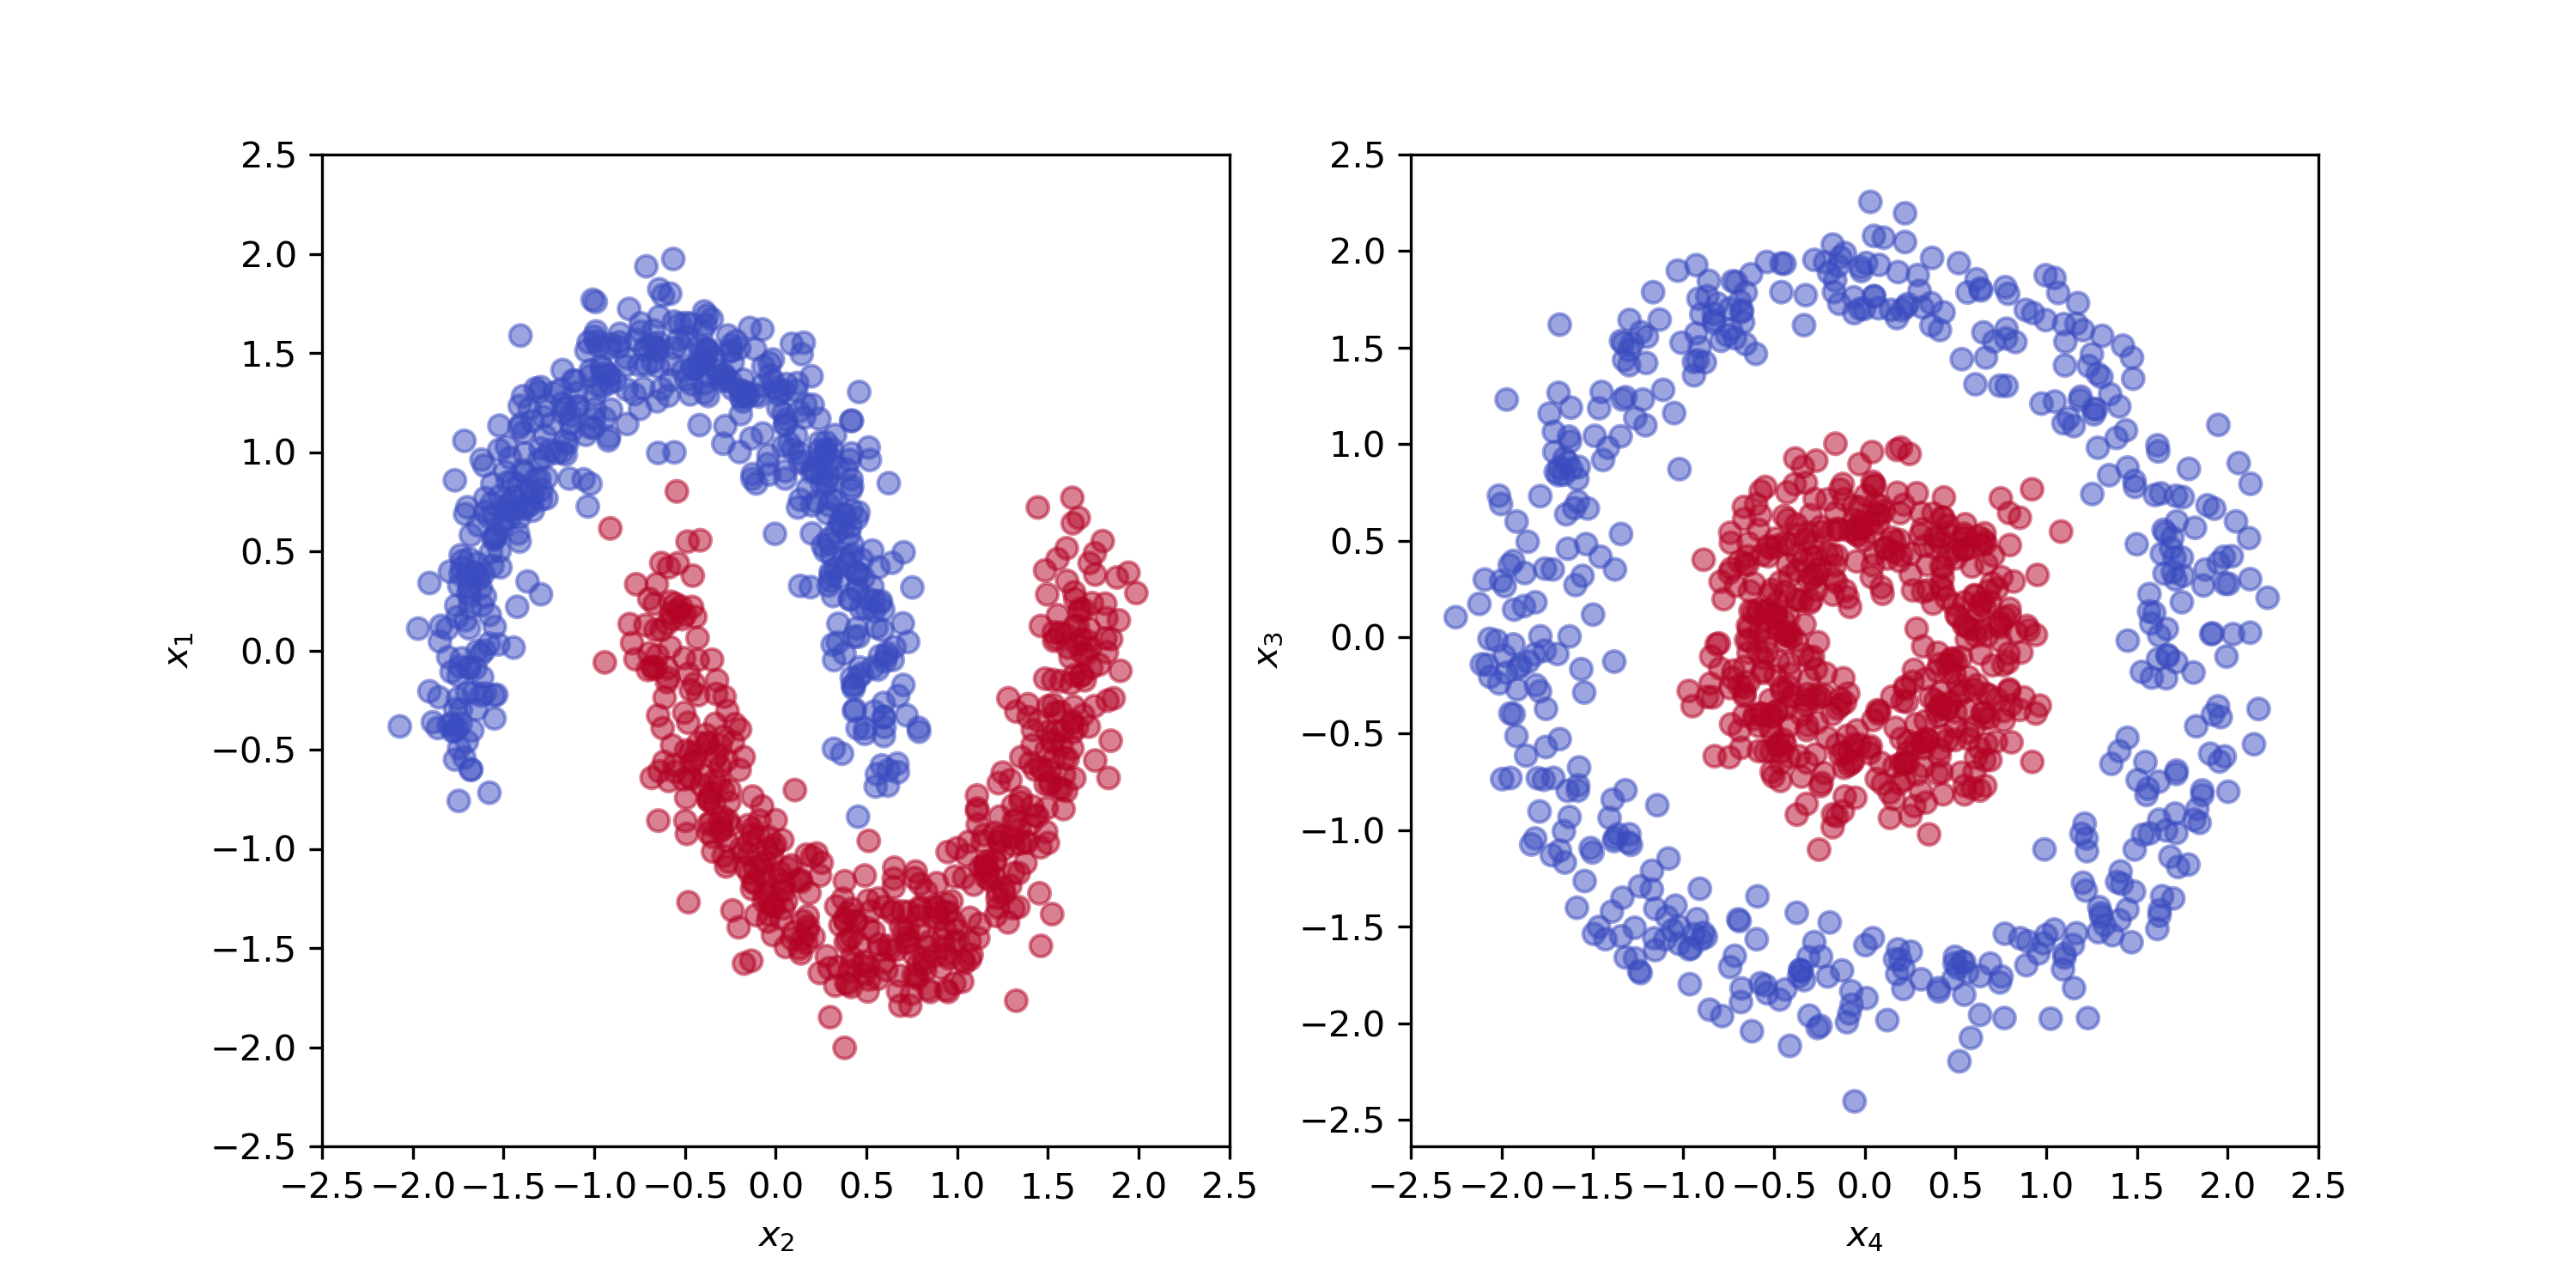
\includegraphics[width=1.0\linewidth]{moons-circles.png}
    \caption{
        This figure depicts the two dataset. 
        On the left, the `Two Moons Dataset' is displayed. 
        On the right, the `Circles' dataset. 
        The datasets are normalized to have zero mean and unit variance in each feature.
    }\label{fig:moons_circles}
\end{figure}

The two selected datasets are the two moons dataset and the Circles dataset, depicted in figure~\ref{fig:moons_circles}.

Both datasets can be interpreted as a two dimensional plane, where the inputs describe coordinates of points on the plane. 
The labels of the dataset relates to the class.
Each point belongs to one class: red or blue.
Concretley, let $\begin{pmatrix} x_1 & x_2 \end{pmatrix}$ be the inputs of the two-moons dataset and $y_1 \in \{0,1\}$ the class label.
The data is generated by creating two half circles of evently spaced points, with a radius of $1$.
One of the half circles is rotated by 180 degrees and shifted by $0.5$.
Gaussian noise with a mean of $0$ and standard deviation of $0.1$ is added to each point in the dataset.

Let $\begin{pmatrix} x_3 & x_4 \end{pmatrix}$ be the inputs of the cirlces dataset and $y_2 \in \{0,1\}$ the class label.
The data is generated by creating evenly spaced points on the inner and outer circle. 
The center of both circles is at $(0,0)$ and the radius of the outer circle is $1$.
The radius of the inner circle is set to be $0.35$.
Gaussian noise with a mean of $0$ and standard deviation of $0.1$ is added to each point in the dataset.
The values of noise the size of the inner cirlce are selected, such that the points do not mix among the circles.

The classic machine learning library `scikit-learn' is used to generate the data. 
The following code snippet demonstrates how the data was generated.
The described sampling strategy for the datasets relates to the content of the functions of `scikitlearn', `makemoons' and `makecircles' respectively.

\begin{figure}[ht]
\centering
\begin{minipage}{\linewidth}
\begin{lstlisting}[
    language=Python,
    captionpos=b, 
    label={code:data},
    caption={
    This code snippet contains python-flavoured pseudo code.
    It depicts the procedure of generating the Moons-Circles dataset.
    },
]
# the sklearn package is used to generate the datasets
import sklearn 

# generates a shuffled set of data points with labels
circles_x, circles_y = sklearn.datasets.make_circles(
    n_samples=2000, 
    noise=0.1, 
    factor=0.35
)

# generates a shuffled set of data points with labels (1000,)
moons_x, moons_y = sklearn.datasets.make_moons(
    n_samples=2000, 
    noise=0.1
)

# Note: 
#   - moons_x and circles_x are numpy arrays of shape (1000, 2) 
#   - moons_y and circles_y are numpy arrays of shape (1000, ) 

# concatenated data points have shape (1000,4)
circles_moons_x = concatenate(circles_x, moons_x)

# concatenate labels have shape shape (1000,2)
circles_moons_y = concatenate(circles_y, moons_y)

# split the dataset in half
x_train, x_test, y_train, y_test = sklearn.model_selection.train_test_split(
    circles_moons_x, 
    circles_moons_y, 
    test_size=0.5, 
)

# scale data to zero mean, unit variance, based on training data
scaler = sklearn.preprocessing.StandardScaler().fit(x_train)
x_train = scaler.transform(x_train)
x_test = scaler.transform(x_test)

(x_train, y_train) # the training data
(x_test, y_test) # the test data


\end{lstlisting}
\end{minipage}
\end{figure}

Since ranges of values of the datasets are different due to their sampling strategy, each feature is normalized individually to have zero mean and unit variance.
The final, normalized dataset is depicted in figure~\ref{fig:moons_circles}

To create a single dataset out of the two seperate datasets, the input features as well as the labels are concatenated.
Concretely, one sample of the concatenated dataset $\hat x$ contains one randomly selected sample from the two moons dataset and one randomly selected sample from the circles dataset.
The label $\hat y$ of the sample $\hat x$ also consist of the respective concatenated labels.
$$\hat x = \begin{pmatrix} x_1 & x_2 & x_3 & x_4 \end{pmatrix}$$
$$\hat y = \begin{pmatrix} y_1 & y_2 \end{pmatrix}$$

In this way, the whole dataset is concatenated.
Afterwards, the dataset is randomly split in half into a training set and a test set.
The result is a training set and a test set with 1000 samples each.

This dataset contains two seperate and indepdent tasks.
For each task, only the respective inputs contain valuable information for the prediction of the class.

\begin{figure}[ht]
    \centering
    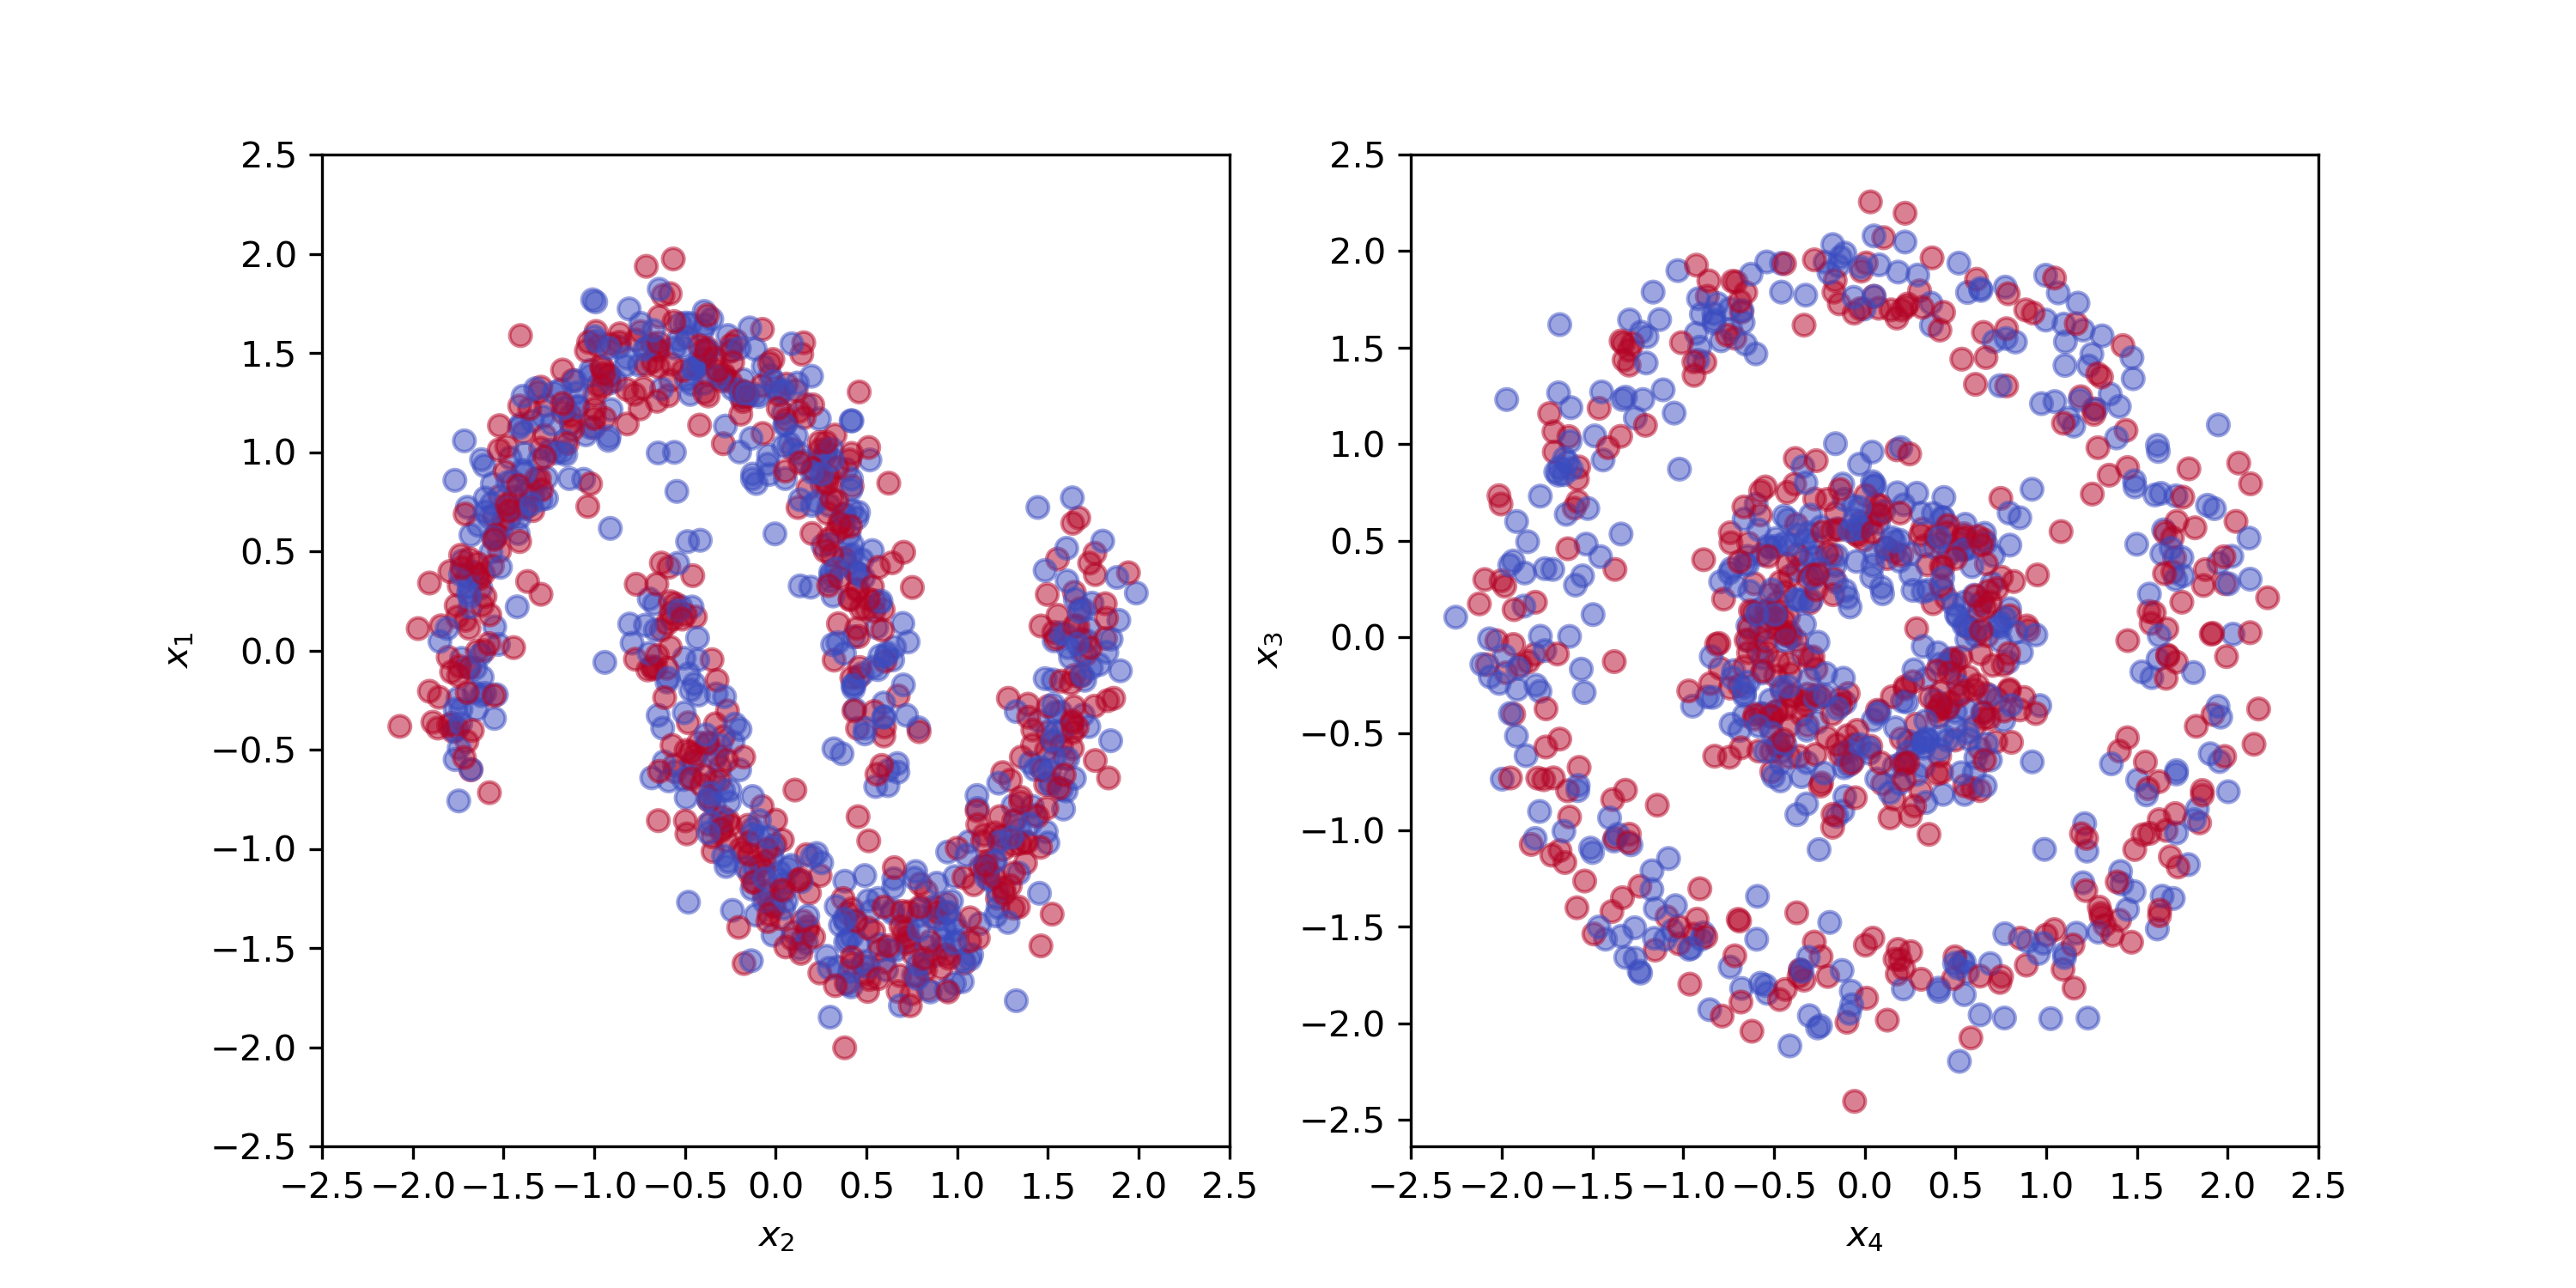
\includegraphics[width=1.0\linewidth]{moons-circles-inverted.png}
    \caption{
        This figure depicts the moons dataset on the left, where the colors are the labels of the circles dataset.
        On the right, the circles dataset is depicted, with the colors representing the class of the moons dataset.
    }\label{fig:moons_circles_inverted}
\end{figure}

This is demonstrated in figure~\ref{fig:moons_circles_inverted}.
The data is the exact same data as is visible in figure~\ref{fig:moons_circles}. 
However, one dataset is displayed with the labels of the other dataset and vice versa.
Concretely, on the left side, the coordinates represent $x_1$ and $x_2$, but the colors refer to $y_2$.
On the right side on the other hand, $x_2$ and $x3$ are displayed with the colors defined by $y_1$.
There is no clear visible pattern discernible from these dataset given on their own.


\section{The Network}
The neural network used to train on this task was inspired by the original lottery ticket experiments \autocite{DBLP:conf/iclr/FrankleC19}. 
A fully connected feed forward neural network was used.
The network has four input neurons, two output neurons and between one and three hidden layers.
Throughout the thesis, experiments with varying numbers of hidden layers are conducted.
The input neurons correspond to $x_1, x_2, x_3, x_4$ defined in the previous section~\ref{sec:independece_dataset}.
The network outputs correspond to $y_1$ and $y_2$.

As non-linearity, the Rectified Linear Unit (ReLU) is used.
The gaussian Xavier-initialization~\textcite{XAVIER-GLOROT} was used by \textcite{DBLP:conf/iclr/FrankleC19} in the original experiments.
However, the authors did not justify their decision.
Since the networks use the ReLU activation function, gaussian Kaiming-initialization~\autocite{KAIMING-HE} will be used as the initialization technique.
The initialization of the biases is not mentioned by \textcite{DBLP:conf/iclr/FrankleC19}.
Throughout this thesis, biases of the network are initialized with zero.
The random initialization of the weights is explicitly controlled via a random seed, to enable reproducibility.
Throughout the thesis, experiments are repeated with three to five different seeds for more robust results.

For the Moons-Circles dataset, the binary cross entropy loss function is used.
It is calculated seperately for every output feature of the network.

\section{The Training Process}
With the dataset and architecture described above the aim was to find lottery tickets.
To accomplish this task, the classic Iterative Magnitude Pruning algorithm described in refIMP was employed used by \textcite{DBLP:conf/iclr/FrankleC19} in the original lottery ticket experiments.
The weights are rewound to $0$.
\textcite{LinearModeConnectivity} demostrated that the LeNet architecture trained on MNIST is stable at initialization, meaning that lottery can be found rewinding the weights to $t=0$ (the value at initialization). 
Since the model and dataset in our case is significantly less complex, it is assumed that the resetting the weights to zero is sufficient to discover lottery tickets.

As pruning criterion, the original magnitude pruning used by \autocite{DBLP:conf/iclr/FrankleC19} is used. 
Since \autocite{DBLP:conf/nips/ZhouLLY19} showed that magnitude pruning is amongst the best performing criteria, it was selected due to its simplicity and widespread usage.
Biases are not pruned.

Contrary to \autocite{DBLP:conf/iclr/FrankleC19} where layerwise pruning is applied, the network is pruned globally.
Concretely, the pruning criterion is applied to all weights at once.
This enables the algorithm to `select' the sparsity for each layer on it's own, resulting in less assumptions that have to be made.

One training run consists of $L$ pruning levels. 
At each pruning level, $p$-percent (pruning rate) of the remaining prunable parameters are set to zero.
The number of prunable parameters equals the number of weights that have not yet been pruned.
After $L$ pruning levels, the number of prunable parameters is termed the `pruning target'.

Over the pruning levels, the number of prunable parameters goes from the initial number to the pruning target.
The sequence of prunable paremters is termed `parameter trajectory'.
A parameter trajectory can be uniquely defined by 3 out of the following 4 values:
\begin{itemize}
    \item prunable parameters at initialization
    \item pruning levels
    \item pruning rate
    \item pruning target
\end{itemize}

Different combinations can be useful for different scenarios.

The networks are trained with the ADAM optimizer.
The learning rate is set to 0.001 and a batch size of 64 is used.
These values were selected based on their effectiveness in preliminary experiments. However it is important to note that they are somewhat arbitrary and may be suboptimal.
Further, throughout the experiments, early stopping is used to reduce the computational time.

As a pruning target for the experiments with the Moons-Circles dataset, values between 100 and 120 were selected.
The pruning target is, in many experiments, derived from the model architecture which will be described in detail in a later chapter.
The pruning target refers to the number of unpruned weights after all pruning iterations are completed.
This however does not mean, that all the unpruned weights are of use to the network.
The number of active weights, which will be discussed in detail in this chapter, can be significantly lower than the pruning target.
It refers to the weights that actually influence the output of the network.

\begin{minipage}{\linewidth}
\begin{lstlisting}[language=Python,caption={This code snippet contains python-flavoured pseudo code.
    It depicts the general procedure of iterative magnitude pruning used for the experiments in this thesis.},captionpos=b, label={code:imp}]

    # given
    model: torch.nn.module  # the freshly initialized model 
    parameter_trajetory: List[int] # defines the pruning process
    train_data, test_data  # data for training
    
    # save state to reinitialze after pruning
    initial_model_state = save_model_state(model)
    
    parameter_count = parameter_trajetory[0]
    for target in parameter_trajectory:

        # no pruning before the first training
        if not first_iteration:

            # the number of parameters to prune from the model
            pruning_amount = parameter_count - parameter_target
            parameter_count = parameter_target

            # prune the model 
            prune(model, pruning_amount)

            # reinitialize the remaining values with initial values
            reinit(model, initial_model_state)

        # actual training and evaluation
        train_loss = train(model, train_data)
        val_loss, val_accuracy = evaluate(model, test_data)

        # transform to a graph and see if it split or degraded
        dag = transform_to_digraph(model)
        evaluate_dag(dag)

        # the run is stopped when graph is degraded 
        # to limit training time
        if graph_degraded:
            break

        # early stopping is used to limit training time
        if early_stopping:
            break
    \end{lstlisting}
\end{minipage}

In the code snippet~\ref{code:imp} the algorithm for iterative magnitude pruning is depicted in python-flavoured pseudo code.
Details have been omited for readability.
Imporantly, the order of the commands are outlined to give a better sense of the algorithm.
The algorithm requires a model, parameter trajectory and data.
The model refers to the freshly initialized neural network.
The parameter trajectory, as described earlier in this paragrah, refers to the number of weights the network should have at every pruning level.
The difference between two neighbouring entries in the parameter trajectory gives the number of parameters to prune in the given level.

\section{Network Splitting}
Since the goal of the experiments is to show if two seperate networks for inside the initial network, a mechanism to check if this is the case is needed.

Before the first pruning level, the network is converted into a Directed Acyclic Graph $\mathcal{G}$.
This graph representation is maintained throughout the pruning levels and updated after each level.

In the first step, each neuron is converted to a node in the graph.
Then each weight is converted into an edge that connects one node from the previous layer to the next layer.
All nodes, with the exception of the input layer, have biases associated with them.

Four categories are defined for the nodes and edges in the graph.
\begin{enumerate}
    \item active parameters  \\
    Nodes or edges in the graph that are connected to at least one input node and at least one output node.
    \item inactive parameters \\
    Nodes or edges that are not connected to any output node. They do not influence the result of the network and they do not receive gradients. They can be removed.
    \item pruned parameters \\
    Nodes or edges that have been masked out by the pruning algorithm.
    \item zombie parameters \\
    Nodes or edges that are not connected to any input node, but are connected to at least one output node.
\end{enumerate}
Before the first pruning level, all nodes and edges are classified as `active parameters'.
In the next step, each parameter in the graph will be assigned a category.
First, the newly pruned weights are extracted from the pytorch module.
Each edge in the graph that was pruned, is assigned that category.

Then, a subgraph $\mathcal{G}_{unpruned}$ is created, excluding all pruned weights.
On $\mathcal{G}_{unpruned}$, inactive nodes and edges are found and assigned their category.
All nodes that are not connected to any output node are classified as inactive.
Further, all edges that are connected to an inactive node are classified as inactive.

Then, a subgraph $\mathcal{G}_{active/zombies}$ is created, excluding all pruned and inactive weights.
On $\mathcal{G}_{active/zombies}$ zombie parameters are found and assigned to their category. 
All nodes that are not connected to any input feature are classified as a zombie parameter. 
Furhter, all edges that are connected to a zombie node are classified as a zombie parameter.

An active subgraph $\mathcal{G}_{active}$, where all nodes are connected to at least one input node and at least one output node.

\subsection{Matching Networks and Tasks}
The active graph $\mathcal{G}_{active}$ is used to find seperate components in the graph.
Conveniently, this can be done with a single networkx function.
\begin{lstlisting}[language=Python]
import networkx as nx

# G : nx.DiGraph
subnetworks = [
    G.subgraph(c) 
    for c in nx.connected_components(G.to_undirected())
]
\end{lstlisting}

Each node or edge of $\mathcal{G}_{active}$ is contained in exactly one of the subnetworks.
There is no overlap between the subnetworks.
Next, the subnetworks are matched to the tasks, which are defined by the dataset.
For each subnetwork and each task in the dataset, the inputs and outputs of the network are compared to the inputs and labels of the task.

Concretely, each task is associated with a set of inputs $T^{(i)}_{in}$ and a set of outputs $T^{(i)}_{out}$.
Further, each subnetwork contains a set of input nodes $N^{(j)}_{in}$ and a set output nodes $N^{(j)}_{out}$.

The intersection of the task inputs and the input nodes of the network denoted input coverage set $C^{(ij)}_{in}$ and output coverage set $C^{(ij)}_{out}$ for the outputs respectively.

$$
C^{(i,j)}_{out} = N^{(j)}_{out} \cap T^{(i)}_{out}
$$
$$
c^{(i,j)}_{out} = \frac{| C^{(i,j)}_{out} |}{|T^{(i)}_{out}|}
$$

$$
C^{(i,j)}_{in}  = N^{(j)}_{in}  \cap T^{(i)}_{in}
$$
$$
c^{(i,j)}_{in} = \frac{| C^{(i,j)}_{in} |}{|T^{(i)}_{in}|}
$$

For evaluating the coverage the the subnetworks as a whole, the number of paths from inputs to outputs are considered.
The total number of paths for a task is given by the product of the cardinatlity of the inputs set and the cardinality of the output set.
Similarly, the number of paths available in the subnetwork is given by the cardinality of theinput coverage set and the cardinatlity of the output coverage set.
The total coverage $c^{(i,j)}$ is defined as the ratio between the products.
$$
c^{(ij)} = \frac{
    | C^{(i,j)}_{in}| * | C^{(i,j)}_{out} |
    }{
    |T^{(i)}_{in}| * |T^{(i)}_{out}|
}
$$
The total coverage is 1 when the task is completely covered by the subnetwork.
It is 0, if either no input or no output of the task is covered by the subnetwork.
It is between 0 and 1, if at least one input and at least one output of the task is covered, but at least one input or output is not covered.
The total coverage is a useful indicator if all inputs and outputs are important, as they are counted equally.
In the case of the Moons-Circles Dataset, the total coverage is used.
For datasets where not all inputs or outputs are necessary or even desired to be used, the input coverage, output coverage or a combination thereof might be a more useful metric.

!!! Maybe move this to dataset.
!!! explain task description in dataset
!!! revise the math part. C is overloaded and number of tasks / subnetworks needs an identified. MAybe J, K and j, k for the running vars.

For instance, given the dataset in ref2, the dataset contains two tasks: the `moons'-task and the `circles'-task. 
The moons-task $T^{(1)}$ is associated with the inputs $T^{(1)}_{in} = \{x_1,x_2\}$ and the output $T^{(1)}_{out} = \{y_1\}$.
The circles-task $T^{(2)}$ is associated with the inputs $T^{(2)}_{in} = \{x_3,x_4\}$ and the output $T^{(1)}_{out} = \{y_4\}$.

The input, output or total coverage can be collected in a matrix $C$ of size $\tau \times j$, where $\tau$ is the number of tasks and $j$ the number of subnetworks. 
$c_{i,j}$ represents the value at the $i$-th row and the $j$-th column and $0 \leq c_{i,j} \leq 1$ holds.
Further, the sum of the matrix is upper bound by the number of tasks.
$$
\sum^{i} \sum^{j} c_{i,j} \leq \tau
$$


Given an unpruned network and a dataset with two tasks the matrix would look like the following 
$$
C = \begin{pmatrix}
    1 \\ 1
\end{pmatrix}
$$
Each task would be completely covered by the same network.
Since the network per definition covers all tasks before the first pruning level, the matrix will be a unit vector with as many entries as there are tasks.

After several pruning iterations, there network might contain two disconnected subnetworks.
In this case, an additional row is added to the matrix.
For instance, let the subnetworks perfectly match the tasks such that every task is completely covered by one subnetwork.
The matrix $C$ might look like the following.
$$
C = \begin{pmatrix}
    1 & 0 \\ 0 & 1
\end{pmatrix}
$$
After further pruning the network, all the connections to one of the input nodes might be pruned.
Then, one of the subnetworks would not be completely covered anymore.
Assuming there are one output node and two input nodes for task 1 and the subnetwork 2 covers all nodes except one input.
The resulting coverage would be 
$$
c^{(1,2)} =  \frac{
    | C^{(1,2)}_{in}| * | C^{(1,2)}_{out} |
    }{
    |T^{(1)}_{in}| * |T^{(1)}_{out}|
} = \frac{1}{2}
$$
and the resulting matrix $C$ would look like the following

$$
C = \begin{pmatrix}
    1 & 0 \\ 0 & 0.5
\end{pmatrix}
$$

If the sum of $C$ is equal to the number of tasks and the number of subnetworks is equal to the number of tasks, then the network is perfectly split.

If the sum of $C$ is equal to the number of task, but there are less subetworks than tasks, the network still needs to split.
The number of splits that are required can is the difference between the number of tasks and the number of subnetworks.

If the sum of $C$ is less than the number of tasks, the network already has lost at one input or output.
This scenario will be referred to as a `degraded' network.
Once a network is degraded, it is impossible that a perfect split is reached.
In the case of the Moons-Circles dataset, the training is stopped as soon as the network is degraded to save computational resources.

(additional)
For mnist, we use the output coverage, since it is expected that the network will come to ignore inputs.
Then the output coverage is used. Also between 0 and 1. Works the same way as with the total coverage in the previous case.

\section{Model Extension}
A technique used to create models that are comparable on the basis of prunable parameters is termed `model extension'. First, the problem is described which model extension is intended to solve, then the technique is described in detail.

To compare networks over pruning levels, a significant quantity is the number of prunable parameters the networks has left at each iteration.
For instance, comparing two networks with 1000 and 1200 prunable parameters in the beginning, 6 pruning levels and a pruning rate of $0.2$, the following parameter trajectories $t_{1000}$ and $t_{1200}$ would form.
$$
t_{1000} = [1000, 800, 640, 512, 409, 327, 262]
$$
$$
t_{1200} = [1200, 960, 768, 614, 491, 393, 314]
$$
The first problem is that the pruning target is not aligned.
Therefore, let the pruning rate be variable and the pruning target is fixed.
The pruning rate can be calculated with 
$$
p = 1 - \sqrt[L]{\frac{T}{P}}
$$
where $L$ is the number of pruning levels, $P$ equals the number of prunable parameters before pruning and $T$ denotes the pruning target.

Let the pruning target be $200$ with 6 pruning levels.
The pruning rates are $p_{1000} = 0.235$ and $p_{1200} = 0.258$ respectively.
The resulting parameter trajectories are as follows.
$$
t_{1000} = [1000, 764, 584, 447, 341, 261, 200]
$$
$$
t_{1200} = [1200, 890, 660, 489, 363, 269, 200]
$$

With this change, the pruning targets are aligned and are comparable.
However at no point during the trajectory values are aligned.
For instance, the network that has $1000$ prunable parameters in the beginning might split after iteration 5, where it has $341$ prunable parameters left. 
The other network might split at iteration after 6, where it has $269$.
However, since they are not aligned one cannot ignore the possibility that the second network would also have split at $341$, but not at $363$. 
The second network would only split earlier if it would split with 22 additional parameters.
When scaling up networks, the intervals at which the had the possibility to split are spaced further from each other, making this effect even more pronounced.

Ideally, different networks would have parameter trajectory that are shared, such that they can be compared at every step.
To achieve this on can `extend the model'.

Let a network with $n$ prunable parameters be the base of the extension.
The network is pruned for any number of pruning levels with a given pruning rate $p$.

TODO write about model extension.

Extending the model means to add parameters to the model, such that pruning it once with the set pruning rate would result in the same number as paraemter


\chapter{Experiments and Results}

\section{Experiments on the Moons-Circles Dataset}
The first round of experiments is dedicated to finding out what conditions are required, such that the network separates.
During a preliminary exploration phase, some scenarios where the network indeed separates were found.
Yet, they were sparse and could not be easily interpreted.
Therefore, in this step, the knowledge gained from the initial experiments was put to use.
A systematic evaluation of the relationship between network size and splitting behavior was conducted.

To enable comparison between networks of different sizes, the network extension technique described in paragraph~\ref{sec:extension} was used.
First, an extensive experiment with a network architecture of $(4,8,8,2)$ was conducted.
To expand the range of the results, two additional experiments were executed, which were slightly smaller to lower computational cost.
One experiment is done on a network with only one hidden layer, concretely with a shape $(4,20,2)$, and the other experiment on a network with three hidden layers, a shape of $(4,4,4,4,2)$.
All other hyperparameters are shared among the three experiments.
The only difference is the pruning target, which is derived from the network architecture.

For all three experiments, the pruning rate was set to $0.32$.
The chosen value, while somewhat arbitrary, was selected by promising results on preliminary tests.
\textcite{LTH} used a pruning rate of $0.2$ in the original experiments for the fully connected feed-forward network trained on the MNIST dataset.
However, with a larger pruning rate, a larger space of network sizes can be covered with the same number of iterations, which is why the larger pruning rate of $0.32$ was selected.

\begin{table}[ht]
    {
    \sffamily
    \caption{
    In this table, the parameter trajectories and the corresponding hidden dimension of the network are displayed for each extension level. 
    The parameter trajectory is in each respective `param' column and the number of hidden neurons per hidden layer is in the column `hidden dim'.
    At the extension level zero, the base model values are displayed.
    }\label{tab:trajectory}
    \begin{tabular}{rrrrrrr}
    \toprule
    Lvl & shape (1) & param (1) & shape (2) & param (2) & shape (3) & param (3) \\
    \midrule
    0 & 20 & 120 & 8 & 112 & 6 & 108 \\
    1 & 29 & 174 & 10 & 160 & 8 & 176 \\
    2 & 43 & 258 & 13 & 247 & 10 & 260 \\
    3 & 64 & 384 & 16 & 352 & 12 & 360 \\
    4 & 94 & 564 & 20 & 520 & 15 & 540 \\
    5 & 138 & 828 & 25 & 775 & 19 & 836 \\
    6 & 202 & 1212 & 31 & 1147 & 23 & 1196 \\
    7 & 297 & 1782 & 38 & 1672 & 29 & 1856 \\
    8 & 437 & 2622 & 47 & 2491 & 35 & 2660 \\
    9 & 643 & 3858 & 57 & 3591 & 43 & 3956 \\
    10 & 946 & 5676 & 70 & 5320 & 52 & 5720 \\
    11 & 1391 & 8346 & 85 & 7735 & 63 & 8316 \\
    12 & 2046 & 12276 & 104 & 11440 & 77 & 12320 \\
    13 & 3009 & 18054 & 127 & 16891 & 94 & 18236 \\
    14 & 4425 & 26550 & 154 & 24640 & 114 & 26676 \\
    15 & 6507 & 39042 & 188 & 36472 & 139 & 39476 \\
    16 & 9569 & 57414 & 229 & 53815 & 169 & 58136 \\
    17 &   &   & 278 & 78952 &   &   \\
    18 &   &   & 337 & 115591 &   &   \\
    19 &   &   & 410 & 170560 &   &   \\
    20 &   &   & 498 & 250992 &   &   \\
    21 &   &   & 604 & 368440 &   &   \\
    22 &   &   & 733 & 541687 &   &   \\
    23 &   &   & 890 & 797440 &   &   \\
    24 &   &   & 1080 & 1172880 &   &   \\
    25 &   &   & 1310 & 1723960 &   &   \\
    \bottomrule
    \end{tabular}
    }
\end{table}

\subsection{Experiments with Two Hidden Layers}\label{two-hidden}
The first experiment was an extensive exploration of different model sizes by extending the network.
The base network, which is the network that is used as a base for extending, has the shape $(4,8,8,2)$.
This architecture has 112 weights, which is also used as the pruning target.
The network architecture indicated by the number of neurons per hidden layer and the respective number of weights are displayed in table~\ref{tab:trajectory}.
The network is extended up to 25 times.
At the extension level 25, the network has a shape of $(4,1310,1310,2)$, with 1.723.960 weights.
The number of extension levels corresponds to the number of pruning levels the network goes through.

Over the course of the pruning levels, the network might separate into two networks or lose one of the inputs or outputs, which is called `degrading'.
For the experiments described here, the training run is stopped as soon as the network degrades to avoid unnecessary computational effort.
After each pruning level, the network is evaluated to check if it is separated or degraded.

When considering all pruning levels, there are four different scenarios for a network:

\begin{enumerate}
\item separated (and not degraded)\\
The network separates at some pruning level. 
It does not degrade at any later level. 
\item separated and later degraded \\
The network splits at some point and has all input and output nodes.
At a later level, the network degrades (it loses at least one input or output).
\item degraded (and not separate before) \\
The network degrades before it can separate.
\item interconnected-not separated and not degraded \\
The network does neither separate nor degrade. 
The result is a single network that contains all input and output nodes of all tasks.
\end{enumerate}

\begin{figure}[ht]
    \centering
    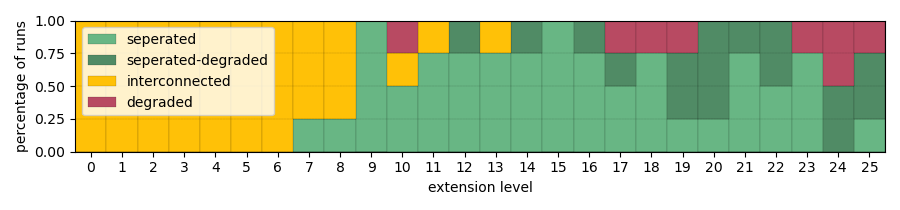
\includegraphics[width=1.0\linewidth]{2-layer-histogram-split-behaviour.png}
    \caption{
        Separate/Degrade Histogram: Two hidden layers
        }\label{fig:2laxer-histogram}
\end{figure}

At each extension level, the runs are repeated with four different seeds for the network initialization.
The results are displayed in figure~\ref{fig:2laxer-histogram}.
The figure is a proportional stacked area chart.
Each scenario described above is encoded with a color.
On the x-axis, the extension levels are shown.
On the y-axis, the percentage of networks in each category can be viewed.
A clear pattern in the data is, that the network separates for the first time with at least 7 pruning levels.
The shape and number of weights at that level are $(4,38,38,2)$ and 1672 respectively, which is $~15$ times the number of weights compared to the base model. 
Starting at shape $(4,57,57,2)$ or extension level 9, which represents an increase of $~32$-times, the majority of the networks separate.
Up until the 6th extension level, none of the networks separate or degrade. 
However, if the network were pruned further, at some point every network would degrade eventually.
Therefore it is also reasonable to assume that some of the networks that are still interconnected after all pruning iterations would separate well if they were pruned to less weights.

Another interesting observation is that only after extension level 10, do the networks begin to degrade.
What follows from the data is the more extension levels, the more likely it is that a network degrades, either before or after it separates.

One possible explanation for this is that at each pruning level, a certain number of `inactive weights' are produced.
As noted in \autocite{HanEtAl15, AllAlivePruning}, this is a known phenomenon.
However, since no regularisation is used in these experiments, the inactive weights do not decrease in magnitude.
Rather, they are frozen with their last value.
If more inactive parameters are created at each pruning level than pruned, the percentage of inactive weights in the network grows over the iterations.
Therefore, the more pruning levels the network experienced, the less of its available, unpruned parameters are active.
This effectively makes the network smaller, which in turn makes it more likely to separate or degrade.

\begin{figure}[ht]
    \centering
    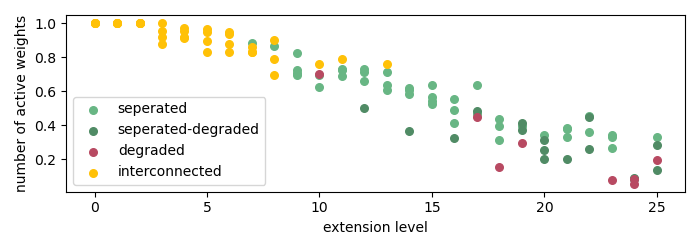
\includegraphics[width=1.0\linewidth]{2-layer-compund-damage.png}
    \caption{
        Active weights at the end of the training run: Two hidden layers
    }\label{fig:collateral_damage}
\end{figure}

This effect is visible in figure~\ref{fig:collateral_damage}.
The colors are encoded in the same way as in figure~\ref{fig:2laxer-histogram}.
Each dot represents a single training run. 
On the x-axis, the extension level is displayed.
On the y-axis, the number of active weights after the last pruning level is displayed.
A clear pattern emerges, showing a correlation between the number of pruning iterations and the number of active weights in the final network.
Important to note is that when a network degrades (red), the run is immediately stopped.
Therefore in this graph, the degraded networks might have larger numbers of active weights, compared to other networks that were pruned for the total amount of levels.
However, even with this caveat, a clear trend is visible.
The more pruning levels the network experiences, the smaller the percentage of the active network weights.
For some networks that were extended to 20 or more levels, the final percentage of active weights in the network is only $\sim20$ percent, which translates to only $\sim22$ active weights.

Techniques like L1-Regularisation used in \autocite{HanEtAl15} or All-Alive-Pruning \autocite{AllAlivePruning} could counteract this effect of compounding inactive parameters.
However, this is a topic for future research and is not addressed in this thesis. 

\subsection{When do networks separate?}
Do the networks always separate at the same pruning level or with the same number of unpruned parameters?
This question is investigated in the following paragraph.

\begin{figure}[ht]
    \centering
    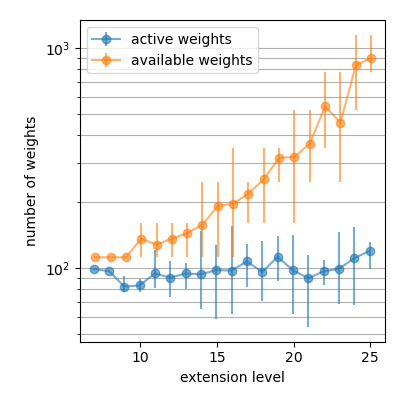
\includegraphics[width=.5\linewidth]{2-layer-active-available-at-split-log.png}
    \caption{
        Active vs. available weights: Two hidden layers
    }\label{fig:2l-active-split}
\end{figure}

Interestingly, when extending the network more, it tends to split into earlier pruning levels.

The figure~\ref{fig:2l-active-split} depicts the number of available/unpruned weights in orange and the number of active weights in blue at the pruning level when the networks separated.
Each dot represents an average of four runs with different seeds.
The error bars indicate the maximum and minimum values of the different runs.
While the number of available weights at the split iteration increases, the number of active weights stays fairly constant.
Logarithmic.
Only the range of extension levels where the network is separated is displayed.
The graph is shown on a logarithmic scale, and the increase follows almost an exponential curve.
The earlier the network separates in terms of pruning levels, the more unpruned weights it has.
However, when looking at the number of active weights the networks have at the iteration they split, the curve does not have the same exponential growth trajectory.
It increases slightly but almost remains flat, covering a narrow range of around 80 to 120 weights.

This data indicates that the number of active weights might be an important quantity to splitting.
Since the active subgraph is indeed the graph on which the splitting is checked, this seems plausible.
 
\subsection{What makes the networks separate?}
As seen in figure~\ref{fig:2laxer-histogram}, the network starts to split at 7 extension levels and a network shape of $(4,38,38,2)$, with 1672 weights.
However, it is not obvious what the main contributor to network splitting is.
To gain a better understanding of that phenomenon an experiment was conducted that compares different combinations of pruning levels, network size, and pruning rate.
For this experiment, four architectures were selected.
One network with shape $(4,31,31,2)$ (extension level 6), which did not separate in any run.
Networks with 38 and 48 hidden neurons (extension levels 7 and 8), where only one in four networks separated.
And finally a network with 57 hidden neurons, where all four runs have separated.
This range of architectures is assumed to encompass a critical area, due to the change in separation behavior.
Further, each of the four architectures was trained with 0 to 10 pruning levels.
The pruning target is fixed at 112, such that all networks end up at the same number of unpruned parameters after the last pruning level.
Therefore, the pruning rate is variable depending on network size and number of levels.
The larger the network, the higher the pruning rate, given a fixed number of iterations.
Each training run with a combination of network size and number of pruning levels was repeated four times, with different seeds for the network initialization.

\begin{figure}[ht]
    \centering
    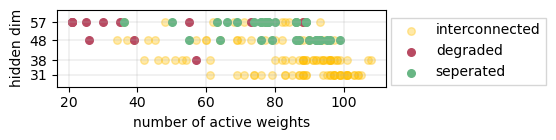
\includegraphics[width=1.0\linewidth]{grid-2-layer-eval-abs.png}
    \caption{Influence of network size: Two hidden layers}\label{fig:grid-1}
\end{figure}

In figure~\ref{fig:grid-1} the impact of network size is demonstrated.
On the y-axis, the size of the network is encoded by its hidden dimension.
On the x-axis, the number of active weights after all pruning levels is depicted.
Each dot represents one training run of the experiment.
The colors denote if the network separated, degraded or stayed connected.
Regarding the two smaller networks with hidden dimensions 31 and 38, none of the networks separated. 
Increasing the number of pruning levels and decreasing the pruning rate did not result in a separated network.
On the other hand, the two larger networks separate numerous times.
These results indicate, that there is a phase change in the ability of the network to separate and that it has to have a certain minimum of overparameterization.

\begin{figure}[ht]
    \centering
    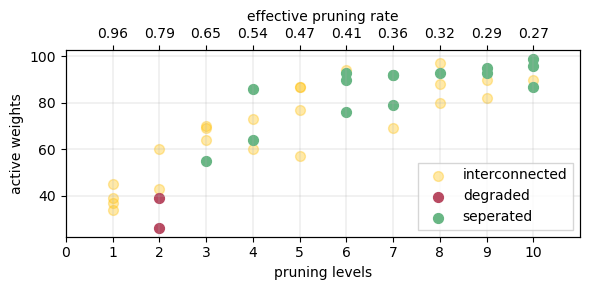
\includegraphics[width=1.0\linewidth]{grid-2-layer-pruning-rate-48-hd.png}
    \caption{Influence of pruning levels: Two hidden layers
    }\label{fig:grid-2}
\end{figure}

To investigate the influence of pruning levels and pruning rate, the separation behavior of the network with hidden dimension 48 is depicted in figure~\ref{fig:grid-2}.
Since the pruning target and the network size are fixed, the pruning rate has to change when increasing the number of pruning levels.
On the bottom x-axis, the number of pruning levels is depicted, and on the top x-axis, is the corresponding pruning rate.
On the y-axis, the number of active weights after all pruning levels is depicted.
With more pruning levels and a lower pruning rate, the network is more likely to separate.
Also, a seemingly contradicting trend to figure~\ref{fig:collateral_damage} is visible, namely that the number of active weights increases with more pruning levels.
The difference to the previous experiment is, that while the number of pruning levels increases in both cases, the pruning rate decreases with more pruning levels in this experiment, which is visible in figure~\ref{fig:grid-2}. In the experiment depicted in figure~\ref{fig:collateral_damage}, the pruning rate is constant, while the network size increases.

However, this data also indicates that there is a certain phase change in the likelihood of the network separating.
Since the pruning rate and the number of pruning levels are two tightly interlinked parameters, it is hard to examine them in isolation.
The largest pruning rate where a network separated was $\sim0.65$. 
With pruning rates lower than $\sim0.41$, the networks consistently separate.
The data indicates that more pruning levels with lower pruning rates are generally favorable to network separation.
\textcite{LTH} already note that iterative pruning leads to smaller lottery tickets than one-shot pruning.
It is reasonable to assume, that the same phenomenon takes place concerning network separation.
Less pruning levels versus lower pruning rates represent a trade-off between favorable conditions and computational cost.

\subsection{Experiments with One and Three Hidden Layers}
To gain a broader picture of the effects shown on the network with two hidden layers, the same experiments were conducted on networks with one and three hidden layers.
As shown in table~\ref{tab:trajectory}, the networks were only extended for 16 levels instead of 25. 
This is due to computational constraints. As the networks get larger and the number of pruning levels is higher, the computational effort increases significantly.

For the network with one hidden layer a base network with shape $(4,20,2)$ was selected.
It has a similar number of weights compared to the base network with two layers.

\begin{figure}[ht]
    \centering
    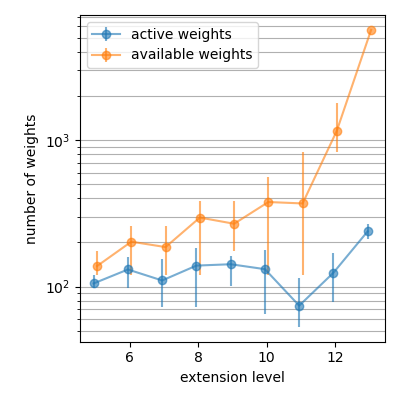
\includegraphics[width=0.5\linewidth]{1-layer-active-available-at-split-log.png}
    \caption{Active vs. available weights: One hidden layer
    }\label{fig:1layer-active}
\end{figure}

\begin{figure}[ht]
    \centering
    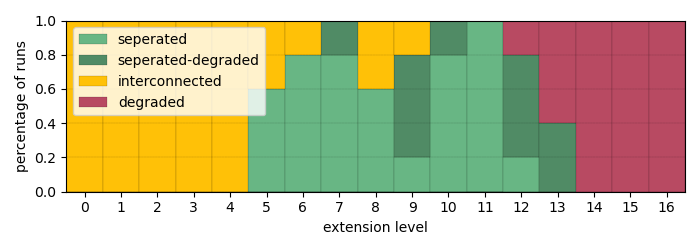
\includegraphics[width=1.0\linewidth]{1-layer-histogram-split-behaviour.png}
    \caption{Separate/Degrade histogram: One hidden layer
    }\label{fig:1layer-histogram}
\end{figure}

In figure~\ref{fig:1layer-histogram}, the same plot as for the two-layer experiment is presented.
On the x-axis, the extension level is displayed. 
Along the y-axis, the percentage of runs per category is shown.
Each color determines the category that the training run belongs to.
A similar trend is visible as in figure~\ref{fig:2laxer-histogram}.
After a certain number of pruning levels and at a certain network size, the networks begin to consistently separate.
Given a few more pruning levels, the networks start to degrade more often, either before or after they separate.
Interestingly, at iteration 12, the network starts to degrade more often before it splits.
Beginning at 14 extension levels, where the networks are the largest, they never split and only degrade.
The reason for this behavior is unknown.
It might be that the networks with more hidden layers also exhibit such behavior at even higher extension levels. 
However, this mystery is not answered in the course of this thesis.

In figure~\ref{fig:1layer-active}, the number of active weights in the network versus the number of available/unpruned weights is compared.
On the x-axis, the number of levels the network was extended to is displayed, which is also the number of pruning levels.
The orange line shows the number of unpruned weights that are available to the network at each iteration where they separate.
The blue line indicates the number of active weights.
The error bars show the minimum and maximum values from the different experiments.
Only the range of extension levels where the network is separated is displayed.
The graph is displayed on a logarithmic scale.

Similarly to the experiment with two layers, the networks separate in earlier iterations when they are larger and have more pruning levels.
This is indicated by the larger number of available weights, which directly correlate with the pruning level.
The number of active weights remains in a fairly tight range between 70 and 120 active weights.

Regarding the network with three hidden layers, the results are similar.
\begin{figure}[ht]
    \centering
    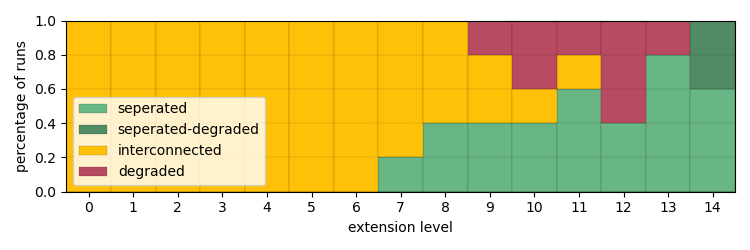
\includegraphics[width=1.0\linewidth]{3-layer-histogram-split-behaviour.png}
    \caption{
        Separate/Degrade histogram: Three hidden layers
    }\label{fig:3layer-histogram}
\end{figure}

\begin{figure}[ht] 
    \centering
    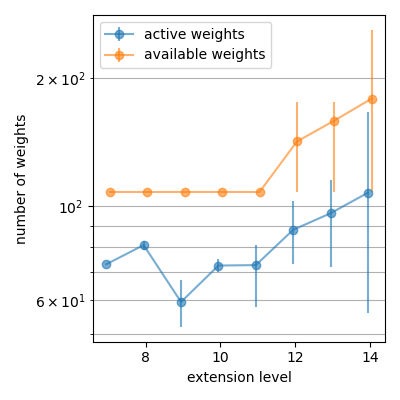
\includegraphics[width=0.5\linewidth]{3-layer-active-available-at-split-log.png}
    \caption{
        Active vs. available weights: Three hidden layers
    }\label{fig:3layer-active}
\end{figure}

In figure~\ref{fig:3layer-histogram} the splitting behaviour is depicted.
A similar effect occurs but unlike the single-layer network, the network does not stop to separate in the range that was tested. 

In figure~\ref{fig:3layer-active} the number of active weights and the number of available weights is displayed.
Only the range of extension levels where the network is separated is displayed.
The networks at extension level 7 until 11 all split at the last pruning level, which can be deducted by the number of available parameters which is equal to the pruning target of 108.
The number of active weights is slightly lower than in the other experiments.
Generally, the same pattern can be seen, with a slightly more pronounced increase in active weights for larger networks.

\subsection{How do networks separate?}
Another open question is, what the process of separation looks like.
In the beginning, it is not yet clear which weight and neuron belongs to which task.
One available option, however, is to view the network from the perspectives of the inputs and outputs.
The input and output features are the only parts of the network that can already be associated with a task when it is fully connected.
This enables us to determine the degree to which the neighboring layers have separated as well.

For instance, regarding the simple Moons-Circles dataset, there are two output neurons.
Each neuron in the penultimate layer has two outgoing connections: one to the Circles-output and one to the Moons-output.
When one of the connections is pruned, the neuron and all its incoming connections are automatically part of the task the unpruned weight is connected to.

The number of neurons in any given layer that are only connected to one of the outputs of one task is denoted $N_{decided}$.
The number of neurons that are connected to both tasks is denoted $N_{undecided}$.
The degree of separation is determined by 
\[
\frac{N_{decided}}{N_{decided}+N_{undecided}}
\]

This calculation can be done from either the side of the inputs or the outputs and it works in the same way.
Only if a layer has at least one neuron that has `decided' to which task it belongs, neurons in the next layer can `decide' as well.

\begin{figure}[ht]
    \centering
    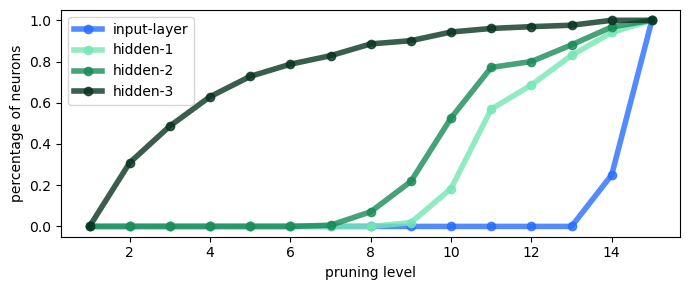
\includegraphics[width=0.9\linewidth]{output-view.png}
    \caption{
    Degree of separation from the output side: Three hidden layers
    }\label{fig:outview}
\end{figure}

\begin{figure}[ht]
    \centering
    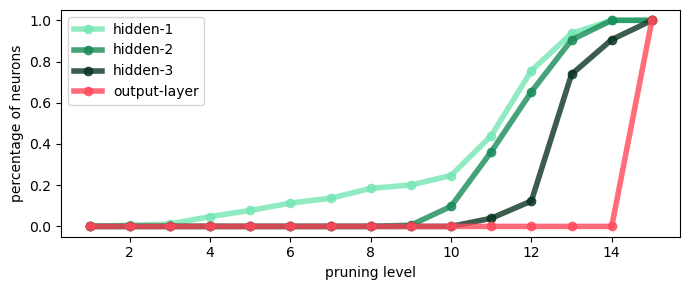
\includegraphics[width=0.9\linewidth]{input-view.png}
    \caption{    
        Degree of separation from input side: Three hidden layers
    }\label{fig:inview}
\end{figure}

In figure~\ref{fig:outview} the degree of separation is displayed for each layer from the view of the outputs.
On the x-axis, the pruning levels are displayed and on the y-axis the percentage of neurons that can be attributed to a task.
The network in this case was taken from the experiment with three hidden layers.
It separates at iteration 15.
In the first iteration, none of the layers were separated.
Already by the second iteration, around $30$\% of the neurons in the last hidden layer (hidden-3) belong to only one task.
This increase in the degree of separation of this layer looks logarithmic.
At iteration 7, where already $\sim80$\% of neurons in the last hidden layer belong to a task, the penultimate hidden layer (hidden-2) starts to separate.
With one iteration delay, the next hidden layer (hidden-1) starts to separate.
It tracks the layer \textit{hidden-2} in its rapid, s-curve-shaped growth.
Only at iteration 14, when over $90$\% of neurons are already attributable to a task, the input layer separates.
In this case, the separation describes the perspective from the outputs.
It does not take into account the knowledge, of which input neuron belongs to which task.

The same network but from the view of the inputs is displayed in figure~\ref{fig:inview}.
On the x-axis, the pruning levels are displayed and on the y-axis the percentage of neurons that can be attributed to a task.
In this case, the separation is significantly slower in the beginning.
After iteration 10, the separation speeds up at iteration 15, the network is completely separated.
The difference in the degree of separation, depending on the point of view, could have several reasons.
It could be that the slower separation is due to the fact, that there are four inputs and only two outputs.
Therefore, for the neurons to be only connected to the inputs of one task, two instead of one weights have to be pruned.
Another possibility is that the weights in the first layer are higher in magnitude than the weights in the last layer.
This would result in stronger pruning in the last layer.
In the course of this thesis, these questions will not be further pursued.

\subsection{Performance of the Separated Networks}
One remaining question is if the networks still perform well when they separate.
Are they better, equal, or worse in terms of the validation loss, compared to the other networks?

\begin{figure}[ht]
    \centering
    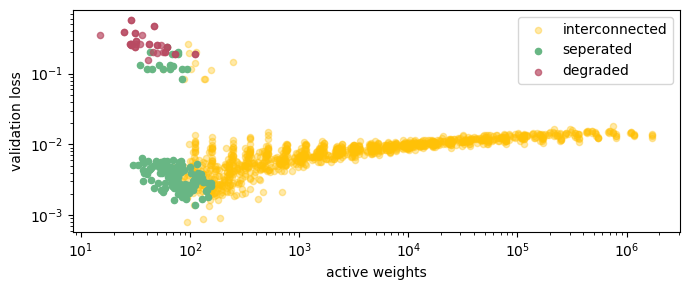
\includegraphics[width=0.9\linewidth]{performance.png}
    \caption{
        Performance at all iterations: Two hidden layers
    }\label{fig:performance}
\end{figure}

To investigate the performance, the validation loss from the experiment with two hidden layers described in paragraph~\ref{two-hidden} was used.
In figure~\ref{fig:performance}, the validation loss is depicted on the y-axis.
On the x-axis, the number of active weights is displayed.
On the y-axis, the validation loss is shown.
Each dot represents a network at one stage.
An experiment with 20 pruning levels is shown with 20 dots in this figure.
The color refers to the state of the network at the iteration.
The color of the point represents if the network was interconnected (yellow), separated (green), or degraded (red) at the iteration the point refers to.
The loss value is calculated after the training and before the pruning of each iteration, as shown in the code snippet~\ref{code:imp}.

The bending line of yellow points demonstrates the consistent performance of the networks during the early iterations.
Likely due to early splitting, the networks remain at a validation loss of around $0.01$.
The loss decreases slightly over the pruning iterations.
A visible cluster of green dots sits at the end of the yellow line.
These dots represent the networks that are separated.
The iterations where the networks are separated are amongst the networks with the lowest loss.
This indicates that the separation of the networks is not merely a consequence of pruning to extremely high sparsities.
Rather, the separated networks still represent a well-performing function, even amongst the best-performing networks overall.

Interestingly, there is a second distinct cluster of networks.
It sits at the same number of active weights, however with significantly higher loss.
This cluster contains interconnected, separated, and degraded networks at seemingly even ratios.
Since the experiments were stopped as soon as a network degraded, the red points refer to losses immediately after the network degraded.
Even though the cluster looks compact along the y-axis it covers a fairly large range between 0.08 and 0.56 loss. These losses correspond to an accuracy of roughly $95$\% and $65$\% respectively.
The separated and interconnected networks still generally inhabit an area with lower loss than the degraded networks.

\section{Experiments on the MNIST-Fashion-MNIST Dataset}
Due to the success of the method in separating the neural network, the same was attempted on the more realistic MNIST-Fashion-MNIST dataset described in paragraph~\ref{sec:mnist}.
The experiments cannot be executed as systematically as before, due to significantly higher computational cost.
However, with experience gained from previous experiments, it was indeed possible to find separated networks.

The hyperparameters are mostly the same as in the previous experiments.
The network is trained with the ADAM optimizer and a learning rate of $0.001$.
Additionally, a larger batch size of 512 is selected, since the data is more diverse and there are significantly more samples.

The dataset includes 1568 input features and 20 output features.
A network with shape $(1568, 784, 392, 20)$ was used for these experiments.
The architecture was selected to resemble the LeNet architecture used in \autocite{LTH} on the MNIST dataset.
The LeNet architecture has a shape of $(784, 300, 100, 10)$.
In preliminary experiments, the networks separated at significantly larger numbers of parameters than in the Moons-Circles experiments.
Therefore, the pruning target was set to 600.
For the training runs, 20 pruning levels were selected, which resulted in a pruning rate of $p=0.3247$, similar to the experiments on the Moons-Circles dataset.
For the first experiments, the data was normalized like the Moons-Circles dataset, namely to zero mean and unit variance.

With the described setup, the network was trained with three different seeds for the weight initialization.
\begin{figure}[ht]
    \centering
    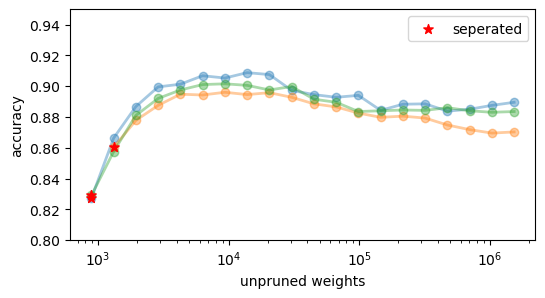
\includegraphics[width=.7\linewidth]{mnist-acc-largest-784-392.png}
    \caption{
        Separation and performance on the MNIST-Fashion-MNIST dataset
    }\label{fig:mnist-acc}
\end{figure}

Figure~\ref{fig:mnist-acc} shows the accuracy of three runs with the same hyperparameters but different seeds on the MNIST-Fashion-MNIST dataset.
On the x-axis, the number of active weights is displayed.
On the y-axis, the accuracy is shown.
Each line represents one run.
The red star indicates where the networks separated.
The iteration where the networks separate is also always the last because after separation occurs, the training is stopped.
When the networks separate, the accuracy already is significantly lower than at the peak.
The best accuracy of a separated network amongst the shown runs is $\sim86$ percent.

\begin{figure}[ht]
    \centering
    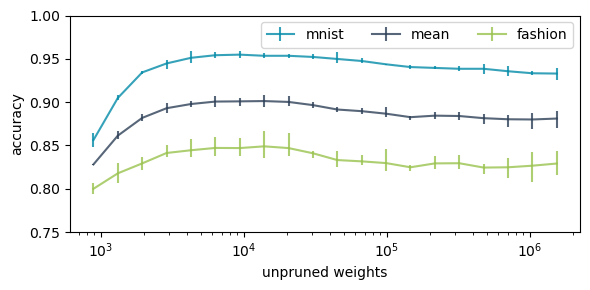
\includegraphics[width=.7\linewidth]{taskwise-acc.png}
    \caption{
        Performance per task
    }\label{fig:taskwise-acc}
\end{figure}

The data shown in figure~\ref{fig:mnist-acc} represents the average accuracy of both tasks.
The data in figure~\ref{fig:taskwise-acc} shows the accuracy of the tasks separately.
Each line is an average of the three runs with different seeds.
The error bars indicate minimum and maximum values.
On the x-axis, the number of active weights is displayed.
On the y-axis, the accuracy is shown.

Since the tasks are not the same, it is to be expected that they do not exhibit the same performance.
The accuracy achieved on the MNIST task is more than $10$ percent higher than on the Fashion MNIST task.
Interestingly, when the number of parameters gets lower, the performance on the MNIST task worsens significantly faster than for the Fashion MNIST task.
The performance of the network is not competitive anymore at the time it separates.
However, the experiments shown here are only preliminary.
The networks indeed separate consistently, and they do far beyond trivial accuracies.
This gives reason to believe, that the separation can be achieved at competitive accuracy with improved hyperparameters or slight adaptations to the training.
This, however, is not pursued in the scope of this thesis.
The separation by itself, at non-trivial accuracy is considered a useful insight into the structure of the network.

\begin{figure}[ht]
    \centering
    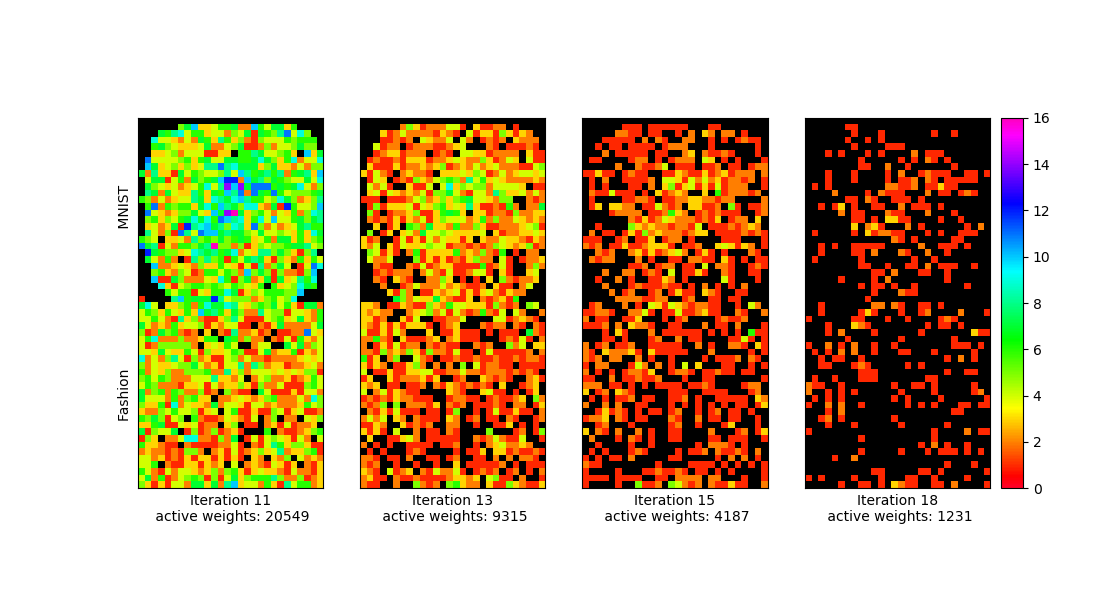
\includegraphics[width=1.\linewidth]{input-connections-iteration-18.png}
    \caption{
        Input pixel heatmap MNIST-Fashion-MNIST
    }\label{fig:input-heatmap}
\end{figure}

The connectivity of the network to the inputs is displayed in figure~\ref{fig:input-heatmap}.
Each figure represents a heatmap of the connectivity to each pixel of the input.
Pixels with no remaining connections are colored black.
The number of input connections per input pixel is displayed.
The heatmap has a shape of $28\times56$ pixels, where the top half represents the MNIST image and the bottom half the Fashion-MNIST image.
On the left, the connections are displayed at iteration $11$, where $\sim20000$ weights are active in the network.
On the top half, many of the pixels on the outer frame have been completely disconnected from the network.
This was also hypothesized by \textcite{LTH} because the outer frame of the MNIST digits is always black and does not contain any information.
On the bottom half where the Fashion-MNIST image would be, there is no frame visible.
This however is also to be expected, because the Fashion-MNIST dataset does not have a padding around the objects that are displayed. 
A larger portion of the image is used.
If the Fashion-MNIST dataset were to be scaled down slightly and padding would be added, a similar pattern would likely emerge.

At iteration 18, where the network is separated, the connectivity is already highly sparse.
Only around half of the input pixels are used and the connectivity to the remaining input pixels is reduced to values between 1 and 3 connected pixels.
This also demonstrates that the separation indeed occurs very late in the pruning process, where the function of the network almost collapses.

\section{Conclusion}
In this section, the experiments on the Moons-Circles dataset as well as the MNIST-Fashion-MNIST dataset were explained in detail.
Over different network sizes, different architectures with varying numbers of hidden layers as well as different pruning rates, the networks separate quite reliably, given the right conditions.
The experiments where the network did not separate either had too small networks, too few pruning levels and too high of a pruning rate.
Also for the more complicated MNIST-Fashion-MNIST dataset, the networks separated with the standard training iterative pruning method.

The results indicate, that iterative magnitude pruning indeed produces lottery tickets with separate subnetworks for independent tasks.

\chapter{Conslusion}

The lottery ticket hypothesis sparked many directions of research in the field of sparse network training and pruning in general.
However, how and why they work remains elusive.

In this thesis, an empirical analysis was conducted on the relationship between the semantic structure of the data and the structure of the sparse lottery ticket subnetwork.
In the experiments conducted, it was shown that networks trained with \textit{Iterative Magnitude Pruning}, produced two independent subnetworks on datasets with independent tasks.
Systematic experiments were conducted on the `Moons-Circles' dataset, a simplistic toy dataset that contains two independent tasks.
Due to the success of the method on the toy task, experiments were also conducted on the `MNIST-Fashion-MNIST' dataset, which is significantly more realistic.
In both cases, neural networks were found to separate with non-trivial accuracy.

\section{Limitations}
The findings of this thesis are empirical, and due the the scope and scale of the thesis, there are numerous untested scenarios.
The experiments were only conducted on toy datasets and on MNIST and Fashion-MNIST which might also be counted as a toy task.
If the findings remain true for larger and more realistic tasks remains to be seen.

\section{Discussion}
The experiments in this thesis demonstrate that iterative magnitude pruning finds independent subnetworks.
This can be valuable for understanding what the structure of lottery tickets represents.
Further, it could also be valuable for machine learning interpretability.
A lottery ticket could be trained and if independent networks occur, it could hint at independence in the dataset.
The same might be true for other types of semantic structure, like feature sharing or compositionality.

\section{Future Work}
An interesting avenue for future research in this line of work would be to examine the numerous other variants for finding sparse subnetworks.
Would they also separate? And if so, would they separate earlier or with better performance still?
Also, an investigation into the influence of things that worked well for lottery tickets, like learning rate schedules and resetting, as well as L1 or L2-regularisation.
Similar to the work in \autocite{BIMT}, other semantic structures of the data might be considered, like compositionality or weight sharing.
Finally, examine the methods on larger and more realistic datasets like CIFAR \autocite{cifar} or ImageNet \autocite{imagenet}, as well as translating the findings into convolutional neural net architectures.

\chapter{Conclusion}


\section{Seminar Conclusion}
Neural Networks have achieved remarkable success in various tasks, however, their increasingly large size leads to high computational and memory requirements.
Neural Network Pruning \autocite{LeCun, OptimalBrainSurgeon, HanEtAl15, PruningFiltersForEfficientConvets} has been proposed to reduce the number of parameters after the network is trained, while maintaining accuracy.
This leads to a reduction in size \autocite{HanEtAl15} and energy consumption \autocite{YangCS17} in the resulting subnetworks during inference.
To increase efficiency during training as well, the smaller networks need to be trained from the beginning. Attempts to train smaller networks discovered by pruning from scratch did not yield convincing results \autocite{HanEtAl15, PruningFiltersForEfficientConvets}.
The Lottery Ticket Hypothesis by \textcite{LTH} has shown that there exist small, well-initialized subnetworks that can be trained in isolation to reach the same accuracy as the unpruned networks. 
In contrast to previous attempts where the subnetwork structure after pruning is randomly reinitialized \autocite{HanEtAl15, PruningFiltersForEfficientConvets}, \textcite{LTH} reinitialize the subnetworks with their respective initial weights from before training.
The subnetwork structure is uncovered by an algorithm called Iterative Magnitude Pruning (IMP).
This paper surveys the recent advancements in finding well-performing subnetworks and the characteristics of these networks. Different approaches for discovering small, well-performing subnetworks are presented, including Supermasks \autocite{Supermasks}, Edge Popup\autocite{DBLP:conf/cvpr/RamanujanWKFR20}, and Gem-Miner\autocite{RareGems}.
\printbibliography[title={Bibliography}, heading=bibintoc]

% additional stuff
\pagenumbering{roman}
\newpage
\listoffigures
\addcontentsline{toc}{chapter}{List of Figures}
\newpage
\listoftables
\addcontentsline{toc}{chapter}{List of Tables}
%\newpage
%\listofmyequations
%\addcontentsline{toc}{chapter}{List of Formulas}
\end{document}